\section{Scalar Yee operators: conventions and finite precision}\label{d:app:model}
\begin{lemma}[Finite stencil and scalar detuning]\label{d:lem:pec}
The matrix in~\eqref{d:eq:maxwell-model} is real symmetric and satisfies $\norm A_2\le16$. A uniform scalar-cell increment $\sigma/\omega^2$ changes $A$ to $A-\sigma I$, including at edges adjacent to the boundary, provided the increment respects the material interval.
\end{lemma}
\begin{proof}
Each retained edge is incident on four faces. Each face has at most four retained edges, so the diagonal of $C_{\rm Y}^{\mathsf T}C_{\rm Y}$ is four and its absolute off-diagonal row sum is at most twelve. Since $1\le(D_\eps)_{ee}\le25$, the diagonal after the mass subtraction lies strictly between zero and four. Both the row and column absolute sums are at most sixteen. Equation~\eqref{d:eq:cell-average} shows that a uniform cell increment adds exactly $\sigma I$ to $\omega^2D_\eps$.
\end{proof}

The geometry in Section~\ref{d:sec:model} fixes the finite operator completely. An oriented edge carries one electric component, and an oriented square face carries the signed sum of its boundary edges. Removing tangential boundary electric unknowns implements the relative-cochain PEC convention. Face rows containing only removed edges may be retained as zero rows. The three terms in~\eqref{d:eq:yee-dimension} count the retained orientations separately.

The four incident cells of every retained electric edge lie inside the physical domain. Thus the mass rule~\eqref{d:eq:cell-average} is the same in the bulk and next to the boundary. A translated finite defect changes the cells in its support by a common increment $v/\omega^2$. Its electric-edge effect is $vW_{\mathcal D}$, where a touched edge has weight equal to the fraction of its four incident cells that belong to the defect. After restricting to touched edges, $W_{\mathcal D}$ is diagonal with entries in $\{1/4,1/2,3/4,1\}$. In particular, $0<w_{\min}\le W_{\mathcal D}\le I$. Defect supports are placed far enough apart that their touched-edge sets are disjoint.

All material and source output is dyadic, with an explicit bit bound. The decoder's finite interface consists of approximations to the real parts of selected electric coordinates, each with a stated absolute error. On the good event, the full inverse bound supplies a polynomial magnitude bound. A fixed number of integer and fractional bits therefore suffices. Outside the good event, the encoder still writes the same bounded-size data and the decoder still reads only its prescribed finite interface; correctness is asserted only on the common good event.

The relative residual target also explains the zero-source convention. If $b=0$, the answer $x=0$ is exact. When an electromagnetic output is required in that case, use a fixed $1\times2\times2$ cell box. It has one retained electric edge, $C_{\rm Y}^{\mathsf T}C_{\rm Y}=4$, and, with $\eps_c=1$, $A=255/64$. This instance is nonsingular with condition number one. The same fixed instance can accompany a precomputed exact answer for the finitely many bounded-size input cases. Use $f=0$ and $\delta=1$, and let the decoder return the stored answer. In particular, the tolerance bound also holds at $m=1$. Those inputs have bounded dimension and bit length under the input assumptions, so their exact processing is a counted fixed cost.

The construction's fixed integer translation basis changes where defects are placed. It does not alter edge lengths, incidence coefficients, or constitutive averaging. A rectangular box containing the transformed balanced layout increases volume by a fixed factor. This property would not follow from a vertex-count bound without the balanced spatial layout established by the logical compiler.

\section{Scalar defects and controlled interactions}
\label{d:sec:physical}

The physical construction uses localized modes as variables and their mutual
interactions as matrix entries. Its main constraint is that the material
parameter is one positive scalar per cell. We therefore cannot prescribe a
general interaction matrix directly. We first construct a fixed dielectric
environment in which a scalar defect supports an isolated mode. We then show
that translated copies of that defect have quantitative interactions of the
form required by the algebraic construction. All objects in this section are
fixed before the input matrix is supplied.

The useful distinction is between an interaction that is small and one that
is both small and reliably nonzero. An upper decay estimate controls
unintended interactions. A lower estimate on selected interactions ensures
that an intended edge remains usable after the other errors are included.
The construction requires both estimates with a strict relation between
their rates.

\subsection{A periodic background with a certified band edge}

Let
\begin{equation}
 A_{\rm per}
   = C_{\rm Y}^{\mathsf T}C_{\rm Y}-\omega^2D_{\varepsilon_{\rm per}},
 \qquad \omega^2=\frac1{64},
 \label{d:eq:physical-periodic-operator}
\end{equation}
be the infinite periodic electric operator, with the cell-to-edge averaging
convention of Section~\ref{d:sec:model}. In an anchor Bloch gauge its fiber is
a finite Laurent matrix
\begin{equation}
 A_{\rm per}(k)=\sum_{\nu\in\mathcal S}A_\nu e^{i\nu\cdot k},
 \qquad A_{-\nu}=A_\nu^T\in\R^{n_{\rm f}\times n_{\rm f}},
 \qquad k\in\mathbb T^3.
 \label{d:eq:physical-laurent-fiber}
\end{equation}
The spectral input to the construction is a unique, simple, nondegenerate
minimum of a positive band. We denote its energy by \(E_c\) and its momentum
by \(k_*\). The point \(k_*\) is invariant under time reversal, so
\(2k_*\in2\pi\Z^3\), and the corresponding eigenvalue has the local expansion
\begin{equation}
 \lambda(k_*+q)
   =E_c+q^THq+O(\abs{q}^4),
 \qquad H>0.
 \label{d:eq:physical-edge-expansion}
\end{equation}
Time reversal and simplicity make the dispersion even. We also require a
complete gap below \(E_c\), a certified separation from the other bands,
and effective bounds on the analytic continuation of the selected band.
These requirements concern the whole Bloch torus.

We supply this spectral input with a fixed inversion-symmetric perturbation
of a period-20 diamond dielectric. The unperturbed scalar cells take values
1 and 12. The perturbed cells have the exact form
\begin{equation}
 \eps_{\mathrm{per}}(c)
   =\eps_{\rm dia}(c)+\frac{p_c}{2^{21}},
 \qquad 0\le p_c\le2046,
 \label{d:eq:physical-exact-material}
\end{equation}
where the integer table \(p_c\), rather than its numerical generator,
defines the material. There are 2000 cells in a primitive FCC cell and
8000 in the conventional cubic cell. The certificate verifies the lattice
translations and scalar inversion symmetry directly.

The certificate has two complementary parts. Near each of the four
inequivalent primitive \(\mathrm{L}\) points, an exact polynomial spectral test proves
\begin{equation}
 \lambda_{\mathrm{low}}(\mathrm{L}+q)-\lambda_{\mathrm{low}}(\mathrm{L})
   >\frac{\abs{q}^2}{600},
 \qquad 0<\abs{q}\le\frac1{20},
 \label{d:eq:physical-local-minimum}
\end{equation}
in Cartesian reciprocal coordinates. Exact eigenvalue enclosures order the
four center values and select \(\mathrm{L}_{++-}\). On the complement, interval
matrix certificates and an analytic treatment of the \(\mathrm{\Gamma}\) region
exclude any lower positive-band value. Section~\ref{d:app:certificate}
gives the assembly, including the distinction between symmetries of the
comparison material and those of the perturbed material.

In the conventional cell, all four primitive \(\mathrm{L}\) points fold to the
same reciprocal class. We use the representative \(k_*=(\pi,\pi,-\pi)\),
consistent with \(\mathrm{L}_{++-}\). The strict ordering of their energies preserves the
simplicity of the lowest eigenvalue under this folding. In radian Bloch
coordinates the certificate yields
\begin{equation}
 2H=\lambda''(k_*)>\frac1{12000}I,
 \qquad g_-=\frac1{128},
 \qquad h_{\mathrm{mat}}=12.
 \label{d:eq:physical-certified-constants}
\end{equation}
Here \(g_-\) separates the edge from all lower bands, and
\(\max\eps_{\mathrm{per}}+E_c/\omega^2<25-h_{\mathrm{mat}}\) leaves material
headroom for the uniform shift and the scalar defects. The finite checks
are part of a computer-assisted proof; the analytic implications below
apply to any periodic finite-range operator with the stated edge data.

\subsection{A scalar defect with a useful isolated mode}

Let \(\mathcal D\) be a finite set of scalar cells. Let \(Q_{\mathcal D}\)
restrict an electric field to affected edges, and let \(W_{\mathcal D}\) contain the
fractions of incident cells belonging to \(\mathcal D\). Its diagonal
entries lie in \(\{1/4,1/2,3/4,1\}\). Increasing every cell of
\(\mathcal D\) by \(v/\omega^2\) changes the electric operator by
\(-vK_{\mathcal D}K_{\mathcal D}^T\), where
\[
 K_{\mathcal D}=Q_{\mathcal D}^TW_{\mathcal D}^{1/2}.
\]
This representation retains the scalar-cell constraint exactly.

For \(0<\xi<g_-/2\), define the shifted background and its finite
compression by
\begin{equation}
 A_\xi=A_{\rm per}-E_\xi I,\qquad E_\xi=E_c-\xi,
 \qquad
 S_\xi=K_{\mathcal D}^TA_\xi^{-1}K_{\mathcal D}.
 \label{d:eq:physical-compression}
\end{equation}
Let \(\Phi_*\) be the real extended edge Bloch field, normalized to have
squared norm one per period cell, and put
\(\Phi_{\mathcal D}=K_{\mathcal D}^T\Phi_*\). In three dimensions the finite matrix
\(S_\xi\) has a limit as \(\xi\downarrow0\), even though the infinite
edge operator has no bounded inverse. The leading correction is
\begin{equation}
 S_\xi=S_0-
   \frac{\sqrt{\xi}}{4\pi\sqrt{\det H}}\Phi_{\mathcal D}\Phi_{\mathcal D}^T+O(\xi).
 \label{d:eq:physical-square-root}
\end{equation}
This expansion is the link between the band edge and the selected defect
mode. Its proof comes from integrating the quadratic band singularity in
three dimensions; Section~\ref{d:app:edge} gives the error estimates.

Choose \(\mathcal D\) to contain all cells of a sufficiently large fixed
cube. Coherent addition of its Bloch amplitudes gives
\begin{equation}
 \frac{\Phi_{\mathcal D}^TS_0\Phi_{\mathcal D}}{\norm{\Phi_{\mathcal D}}^2}
   \ge c_{\mathrm{cube}}L_{\rm cube}^2-\frac1{g_-},
 \label{d:eq:physical-cube-growth}
\end{equation}
where \(L_{\rm cube}\) is the number of period cells along each interior side.
Consequently \(S_0\) has a sufficiently large eigenvalue whose eigenspace
overlaps \(\Phi_{\mathcal D}\). The rank-one square-root term in
\eqref{d:eq:physical-square-root} selects a simple branch even when that
limiting eigenvalue is degenerate. For sufficiently small fixed \(\xi\),
we obtain a positive simple eigenpair \((\mu_\xi,u_\xi)\) with
\[
 \Phi_{\mathcal D}^Tu_\xi\ne0.
\]
The reciprocal \(v_*=\mu_\xi^{-1}\) is small enough to fit within the
material headroom. Birman--Schwinger algebra then gives a one-dimensional
kernel of
\(A_\xi-v_*K_{\mathcal D}K_{\mathcal D}^T\), with field
\(A_\xi^{-1}K_{\mathcal D}u_\xi\). The background gap and finite
stencil imply exponential localization. A fixed two-sided interval around
\(v_*\) remains admissible, allowing subsequent algebraic calibration.

The nonzero overlap is more than an existence property of the mode. It
prevents the leading interaction amplitude from vanishing at the complex
momenta that determine long-range transmission.

The effective algebra can already be seen before the finite-domain
estimates are introduced. For disjoint translated defects, let
\(K_{\rm all}=[K_1\ \cdots\ K_J]\) and
\(V_{\rm d}=\operatorname{diag}(v_1I,\ldots,v_JI)\).
If
\[
 (A_\xi-K_{\rm all}V_{\rm d}K_{\rm all}^T)E=f,
\]
then the defect moments \(z=V_{\rm d}K_{\rm all}^TE\) satisfy the exact
finite system
\begin{equation}
 \bigl(V_{\rm d}^{-1}
       -K_{\rm all}^TA_\xi^{-1}K_{\rm all}\bigr)z
   =K_{\rm all}^TA_\xi^{-1}f.
 \label{d:eq:physical-effective-moments}
\end{equation}
In the selected mode at each defect, the diagonal response is controlled
by \(v_i^{-1}-\mu_\xi\); the off-diagonal response is the corresponding
mode-to-mode interaction. The simple-mode gap controls the effect of
eliminating the other defect channels. This is the origin of the
variables and couplings used by the reduction.

The tunings therefore act through diagonal responses of a structured
effective system. Auxiliary mediator defects convert those responses
into the required signed logical connections. Their calibration uses the
actual directional interactions supplied below. It does not require a
separate material parameter for every matrix entry or every electric
component. The later assembly analysis also includes the corrections
generated by the eliminated channels, the finite boundary, and source
rounding. Equation~\eqref{d:eq:physical-effective-moments} identifies the
mechanism; those bounds establish that the mechanism meets the theorem's
accuracy guarantee.

\subsection{Upper and lower estimates on interactions}

For the selected fixed shift and defect, let
\begin{equation}
 G(\nu)=K_{\mathcal D}^TA_\xi^{-1}\mathcal T_\nu K_{\mathcal D},
 \qquad \nu\in\Z^3,
 \label{d:eq:physical-interaction-block}
\end{equation}
where \(\mathcal T_\nu\) translates by period cells. A complex shift of the full
Bloch integral gives, for any fixed small \(\eta_{\rm t}>0\),
\begin{equation}
 \norm{G(\nu)}
 \le C\exp\!\left[
   -(1-\eta_{\rm t})\sqrt{2\xi}\,
   \norm{(2H)^{-1/2}\nu}\right].
 \label{d:eq:physical-block-upper}
\end{equation}
This controls every interaction channel in the finite defect block.
To obtain a useful lower bound, we examine the selected scalar channel
\(h(\nu)=u_\xi^TG(\nu)u_\xi\).

For a nonzero integer direction \(\upsilon\), let \(\beta_\upsilon\) be the support
point in direction \(\upsilon\) of the small convex level surface
\(E_c-\lambda(k_*+i\beta)=\xi\), and write
\(I_\upsilon=\beta_\upsilon\cdot\upsilon\). The leading asymptotic is
\begin{equation}
 h(d\upsilon)=e^{ik_*\cdot d\upsilon-I_\upsilon d}
 \left[
 \frac{\mathcal N_\xi(k_*+i\beta_\upsilon)}
 {2\pi d\abs{\upsilon}\sqrt{\det Q_{\upsilon,\perp}}}
 +O(d^{-3/2})
 \right].
 \label{d:eq:physical-coupling-asymptotic}
\end{equation}
Here \(Q_{\upsilon,\perp}\) is the restriction of the complex-point dispersion
Hessian to the plane perpendicular to \(\upsilon\), and
\[
 \mathcal N_\xi(k)=
 (\mathcal Ff_\xi)(-k)^T\Pi(k)(\mathcal Ff_\xi)(k),
 \qquad f_\xi=K_{\mathcal D}u_\xi,
\]
uses the Bloch transform \(\mathcal Ff_\xi\) and the analytic rank-one spectral projection \(\Pi(k)\).
For the selected branch, \(\mathcal N_\xi(k_*+i\beta_\upsilon)\) is positive for all
directions once \(\xi\) is sufficiently small. The time-reversal phase in
\eqref{d:eq:physical-coupling-asymptotic} is a sign, so it does not cancel
the magnitude of the leading term.

The proof shifts the entire Fourier torus to the limiting complex
contour before introducing a smooth localization. This order ensures
that every remainder retains the exponential factor
\(e^{-I_\upsilon d}\). A longitudinal pole calculation and a transverse Gaussian
integral then produce the factor \(d^{-1}\). Section~\ref{d:app:green}
provides the contour and remainder argument. Related spectral-edge
asymptotics for periodic elliptic operators provide useful context
\cite{kha2017}; the proof here treats the finite-dimensional Bloch
matrix of the discrete operator directly.

\subsection{A placement lattice with separated interaction rates}

The anisotropy of \(H\) is handled by placing defects on a fixed skew
sublattice. Choose an invertible integer matrix \(B\) close to a large
multiple of \((2H)^{1/2}\). In these placement coordinates, the decay
metric is approximately Euclidean. The comparison
\(\norm{\nu}_2\ge\norm{\nu}_1/\sqrt3\), together with
\(2/\sqrt3>1\), leaves a strict margin between twice the available
upper decay rate and the axial lower decay rates.

\Needspace{15\baselineskip}
\begin{samepage}
\begin{proposition}[Fixed scalar interaction platform]
\label{d:prop:physical-platform}
The certified periodic background admits effectively selectable fixed
data consisting of a dyadically shifted background with spectral gap
\(g_0>0\) at zero, a finite scalar-cell defect, a normalized mode \(u\)
for a positive simple compressed eigenvalue \(\mu\) with complementary
spectral separation \(\gamma_d>0\), and a two-sided admissible scalar
tuning interval with fixed positive upper material headroom.
There are also an invertible integer placement matrix \(B\)
and rational constants \(C_{\rm d},c_{\rm d}>0\), \(0<r_{\rm d},a_{\rm d}<1\), and \(d_0\in\N\), such that
\begin{equation}
 \norm{G(B\nu)}\le C_{\rm d}r_{\rm d}^{\norm{\nu}_1},
 \qquad
 \abs{u^TG(dBe_j)u}\ge c_{\rm d}a_{\rm d}^d
 \quad (d\ge d_0,\ j=1,2,3),
 \qquad r_{\rm d}^2<a_{\rm d}.
 \label{d:eq:physical-platform-bounds}
\end{equation}
All physical cell permittivities remain in \([1,25]\), and the grid metric
and coordinate stretches remain unchanged.
\end{proposition}
\end{samepage}

The strict inequality \(r_{\rm d}^2<a_{\rm d}\) is what makes composition possible.
Intended interactions can be calibrated at a scale proportional to
\(a_{\rm d}^d\), while interactions traversing at least two placement steps are
controlled by \(r_{\rm d}^{2d}\). Their ratio decreases geometrically. The
later construction chooses \(d\) logarithmic in the input size to meet an
inverse-polynomial error budget. The matrix \(B\) specifies positions of
defects; it does not alter the Yee stencil.

\subsection{Effective selection of the fixed platform}

The edge energy \(E_c\) need not be rational. We choose a dyadic operating
shift \(E_\xi<E_c\), set \(\xi=E_c-E_\xi\), and implement the uniform scalar
increment \(E_\xi/\omega^2\). Dovetailing over such shifts and rigorous finite
eigenpair certificates selects the simple branch and its nonzero overlap.
The strict estimates above also permit certified searches for \(B,r_{\rm d},a_{\rm d}\),
the coupling constants, and the large-distance threshold. These searches
terminate and are independent of the sparse input size.

The fixed search may have very large cost. Its termination is established
analytically, and the resulting constants are included in the uniform
asymptotic bound. The finite certificates supply the periodic background
and its edge; the defect and interaction estimates supply the remaining
data needed by the search.

\begin{figure}[htbp]
  \centering
  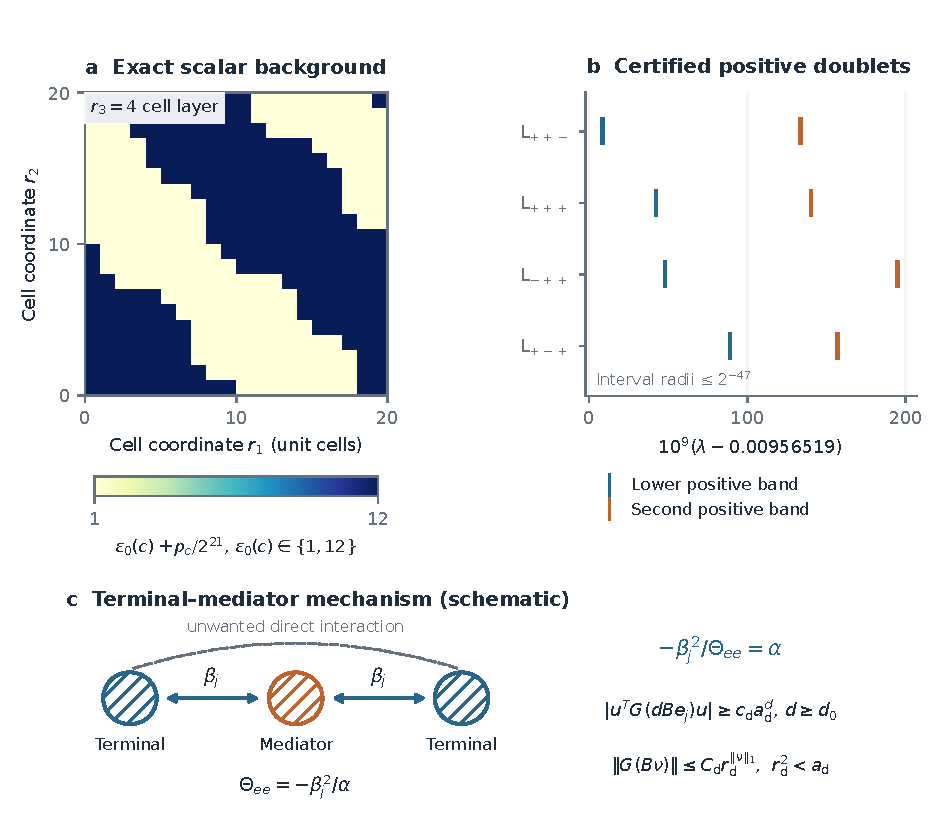
\includegraphics[width=\linewidth]{figures/si/spectral_setting.pdf}
  \caption{Certified spectral setting and analytic interaction mechanism.
  (a) The exact scalar permittivity in cell layer $r_3=4$ (cell centers at
  $r_3=9/2$) of the period-$20$ background. Each pixel is one scalar cell;
  the fixed perturbation is $p_c/2^{21}$, $0\le p_c\le2046$.
  (b) Certified intervals for the two low positive eigenvalues of
  $A_{\rm per}=C_{\rm Y}^{\mathsf T}C_{\rm Y}-D_{\varepsilon_{\rm per}}/64$ at the four
  inequivalent $\mathrm{L}$ points: the subscripts give the signs of their Cartesian
  coordinates $(\pm1/2,\pm1/2,\pm1/2)$ in $\tilde k=k/(2\pi)$.
  Primitive phase coordinates are
  $(\tilde k_x,(\tilde k_x+\tilde k_y)/2,(\tilde k_x+\tilde k_z)/2)$.
  Interval radii are at most $2^{-47}$ and are smaller than the plotted
  line width. The horizontal axis is shifted and scaled as labelled.
  (c) Schematic localized defect supports and the terminal--mediator Schur
  identity. The coupling inequalities use a fixed placement lattice $B$
  and effective constants satisfying $r_{\rm d}^2<a_{\rm d}$, with the useful lower bound
  holding for $d\ge d_0$. The drawing represents the
  analytic construction, without an instantiated defect mode or fitted
  coupling data.}
  \label{d:fig:FIG-2}
\end{figure}

\begin{figure}[htbp]
  \centering
  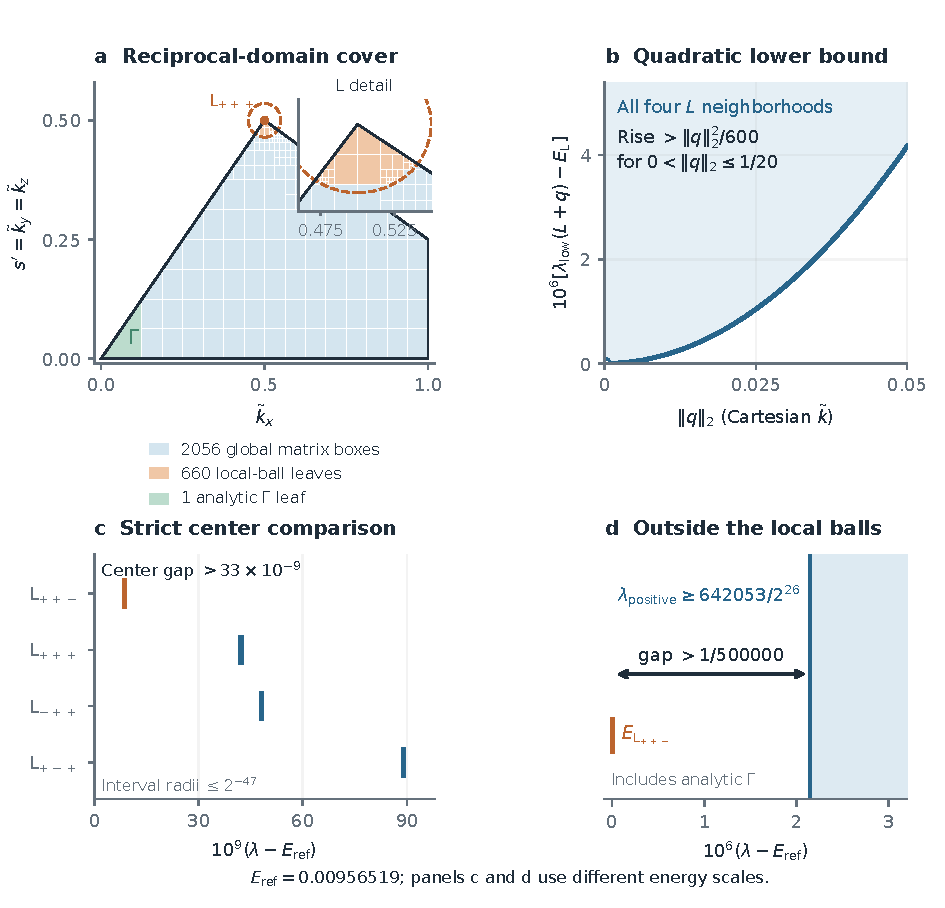
\includegraphics[width=\linewidth]{figures/si/spectral_certification.pdf}
  \caption{Exact certificates and analytic bounds select the global edge.
  (a) The canonical comparator slice
  $(\tilde k_x,\tilde k_y,\tilde k_z)=(s,s',s')$, $0\le s'\le s\le1$,
  $s+2s'\le3/2$, with exact box intersections and a local zoom.
  The legend gives full three-dimensional counts: $2056$ global matrix
  boxes, $660$ leaves wholly inside the radius-$1/20$ local ball, and one
  analytic $\mathrm{\Gamma}$ leaf. The geometric cover also classifies
  $1449$ infeasible leaves, which are not spectral regions and are omitted.
  The dashed ellipse is the ball boundary in this slice. Signed coordinate
  permutations extend the unperturbed comparator; the perturbed material
  has separate certificates for all four inequivalent $\mathrm{L}$ neighborhoods.
  (b) The lower-bound curve $\|q\|_2^2/600$ applies throughout each ball;
  it is not a sampled dispersion curve.
  (c) Exact center intervals select $\mathrm{L}_{++-}$, with every competing lower
  endpoint exceeding its upper endpoint by more than $33/10^9$.
  (d) Outside the four balls, including the analytic $\mathrm{\Gamma}$ region,
  the first positive band is at least $642053/2^{26}$, exceeding the
  selected center by more than $1/500000$. Panels (c) and (d) use the
  same reference energy and different explicitly labelled scales.
  Coordinates are Cartesian $\tilde k$; conventional radian coordinates are
  $k=2\pi\tilde k$, in which the four $\mathrm{L}$ classes fold to the class represented
  by $(\pi,\pi,-\pi)$.}
  \label{d:fig:FIG-3}
\end{figure}

Sections~\ref{d:app:edge}--\ref{d:app:certificate} give the defect,
interaction and spectral arguments. Section~\ref{d:sec:reproducibility}
specifies the finite certificate data.

\section{A scalar defect selected by a simple band edge}
\label{d:app:edge}

This section proves the defect part of
Proposition~\ref{d:prop:physical-platform}. We work with a real, periodic,
finite-range operator whose Bloch matrix has the form
\eqref{d:eq:physical-laurent-fiber}. Assume the edge data of
Section~\ref{d:sec:physical}: a unique simple edge \(E_c\) at a
time-reversal invariant momentum \(k_*\), a lower-band separation \(g_->0\),
and a positive quadratic form \(H\). The coefficients, spectral gaps,
and local analytic estimates are effectively bounded.

\subsection{The compressed resolvent expansion}

Write
\[
 d_\lambda(q)=\lambda(k_*+q)-E_c,\qquad
 d_\lambda(q)=q^THq+O(\abs{q}^4).
\]
After decreasing a fixed radius \(q_0\), choose positive rational constants
\(a_0,a_1,M_4\) such that
\[
 a_0I\le H\le a_1I,\qquad
 \abs{d_\lambda(q)-q^THq}\le M_4\abs{q}^4,\qquad
 \frac{a_0}{2}\abs{q}^2\le d_\lambda(q)\le2a_1\abs{q}^2
\]
for \(\abs{q}\le q_0\). All other spectral contributions have denominators
bounded away from zero near \(E_c\). The real normalized edge eigenvector
\(\phi_*\) extends to the non-square-summable Bloch field
\(\Phi_*(\nu)=e^{ik_*\cdot\nu}\phi_*\).

\begin{lemma}[Square-root edge expansion]
\label{d:lem:physical-square-root}
For the fixed finite defect block \(K_{\mathcal D}=Q_{\mathcal D}^TW_{\mathcal D}^{1/2}\), let
\(\Phi_{\mathcal D}=K_{\mathcal D}^T\Phi_*\) and
\[
 S_\xi=K_{\mathcal D}^TA_\xi^{-1}K_{\mathcal D}.
\]
Then \(S_0=\lim_{\xi\downarrow0}S_\xi\) exists in finite-matrix operator
norm, and
\begin{equation}
 S_\xi=S_0-c_H\sqrt{\xi}\,\Phi_{\mathcal D}\Phi_{\mathcal D}^T+R_\xi,\qquad
 c_H=\frac1{4\pi\sqrt{\det H}},\qquad
 \norm{R_\xi}\le C_{\mathcal D}\xi.
 \label{d:eq:appendix-edge-root}
\end{equation}
The constant and the permitted interval of \(\xi\) can be bounded from
the finite support and the certified edge data.
\end{lemma}

\begin{proof}
Use Bloch measure \((2\pi)^{-3}\,dq\). The selected-band contribution in
the ball \(\abs{q}<q_0\) is
\[
 \int_{\abs{q}<q_0}\frac{\mathcal B(q)}{d_\lambda(q)+\xi}
                    \frac{dq}{(2\pi)^3},
\]
where \(\mathcal B\) is the finite compressed spectral numerator,
\(\mathcal B(0)=\Phi_{\mathcal D}\Phi_{\mathcal D}^T\), and
\(\mathcal B(-q)=\mathcal B(q)^T\). For real \(q\) it is positive
semidefinite. Since \(d_\lambda\) is even, its integral is unchanged by replacing
\(\mathcal B(q)\) with its even part. Analyticity gives
\[
 \norm{\mathcal B_{\mathrm{even}}(q)-\Phi_{\mathcal D}\Phi_{\mathcal D}^T}
 \le C_{\mathcal B}\abs{q}^2.
\]
The singularity \(\abs{q}^{-2}\) is integrable in dimension three, so
the integral at \(\xi=0\) exists. The spectrally separated part also has
a finite limit and changes by \(O(\xi)\).

For the difference of the singular contributions at zero and \(\xi\),
the scalar multiplier is
\[
 \phi_\xi(s)=\frac{\xi}{s(s+\xi)}.
\]
Replacing the even numerator by \(\Phi_{\mathcal D}\Phi_{\mathcal D}^T\) introduces \(O(\xi)\), because
the resulting integrand is bounded by
\(C\xi/(c\abs{q}^2+\xi)\). Replacing \(d_\lambda(q)\) by \(q^THq\) also costs
\(O(\xi)\): the derivative estimate
\[
 \abs{\phi_\xi'(s)}
   =\frac{\xi(2s+\xi)}{s^2(s+\xi)^2}
   \le\frac{2\xi}{s^2(s+\xi)}
\]
combines with the quartic dispersion remainder to give the same integrable
majorant. Extending the remaining quadratic integral to \(\R^3\) adds
only \(O(\xi)\), since its exterior radial tail is bounded by
\(C\xi\int_{q_0}^{\infty}s^{-2}\,ds\).

The change of variables \(q=\sqrt{\xi}\,H^{-1/2}z\) gives
\[
 \int_{\R^3}\frac{\xi\,dq}
 {(q^THq)(q^THq+\xi)(2\pi)^3}
 =
 \frac{\sqrt{\xi}}{\sqrt{\det H}}
 \int_{\R^3}\frac{dz}{\abs{z}^2(\abs{z}^2+1)(2\pi)^3}
 =
 \frac{\sqrt{\xi}}{4\pi\sqrt{\det H}}.
\]
The last equality follows from
\(4\pi\int_0^\infty(1+s^2)^{-1}ds=2\pi^2\).
These estimates establish the expansion and its effective remainder.
\end{proof}

\subsection{A large scalar cube overlaps a large eigenvalue}

Choose an all-cell cube containing every cell incident to the electric
edges of \(L_{\rm cube}^3\) interior period cells, with a fixed indexing margin.
For \(L_{\rm cube}\ge8\), write \(W_\nu\) for the diagonal incident fractions in
period cell \(\nu\). Its support occupies at most \(8L_{\rm cube}^3\) period cells,
and its translation indices can be chosen to satisfy \(\abs{\nu}\le4L_{\rm cube}\).
On the interior cells \(W_\nu=I\). Hence
\begin{equation}
 a_{\rm cube}:=\norm{\Phi_{\mathcal D}}^2=\sum_\nu\phi_*^TW_\nu\phi_*,
 \qquad L_{\rm cube}^3\le a_{\rm cube}\le8L_{\rm cube}^3.
 \label{d:eq:appendix-cube-mass}
\end{equation}
The source \(f_{\mathcal D}=K_{\mathcal D}\Phi_{\mathcal D}\) has period-cell components
\(f_{\mathcal D}(\nu)=W_\nu e^{ik_*\cdot\nu}\phi_*\). Let \(\phi(q)\) be a local normalized
selected-band eigenvector with
\(\norm{\phi(q)-\phi_*}\le C_\phi\abs{q}\). Its source overlap is
\[
 \mathcal N_{\rm cube}(q)
  =\phi(q)^*\sum_\nu e^{-iq\cdot\nu}W_\nu\phi_*,
 \qquad \mathcal N_{\rm cube}(0)=a_{\rm cube}.
\]
The phase and eigenvector changes satisfy
\[
 \abs{\mathcal N_{\rm cube}(q)-a_{\rm cube}}
 \le4L_{\rm cube}\abs{q}a_{\rm cube}+8C_\phi L_{\rm cube}^3\abs{q}.
\]
Choose a fixed rational
\[
 0<q_*\le
 \min\left(q_0,\frac1{64},\frac1{64(1+C_\phi)}\right).
\]
Then \(\abs{\mathcal N_{\rm cube}(q)}\ge a_{\rm cube}/2\) for
\(\abs{q}\le q_*/L_{\rm cube}\). If \(d_{\max}\) satisfies
\(d_\lambda(q)\le d_{\max}\abs{q}^2\), the selected band contributes at least
\[
 \frac{a_{\rm cube}^2}{4}\int_{\abs{q}\le q_*/L_{\rm cube}}
    \frac{dq}{d_{\max}\abs{q}^2(2\pi)^3}
 =\frac{a_{\rm cube}^2q_*}{8\pi^2d_{\max}L_{\rm cube}}.
\]
Other upper-band contributions are nonnegative. The lower bands contribute
at least \(-\norm{f_{\mathcal D}}^2/g_-\), and \(\norm{K_{\mathcal D}}\le1\) implies
\(\norm{f_{\mathcal D}}\le\norm{\Phi_{\mathcal D}}\). Therefore
\begin{equation}
 \frac{\Phi_{\mathcal D}^TS_0\Phi_{\mathcal D}}{\norm{\Phi_{\mathcal D}}^2}
 \ge c_{\mathrm{cube}}L_{\rm cube}^2-\frac1{g_-},
 \qquad c_{\mathrm{cube}}=\frac{q_*}{80d_{\max}}>0,
 \label{d:eq:appendix-cube-rayleigh}
\end{equation}
using \(\pi^2<10\). For any fixed threshold \(\lambda_0\), choose \(L_{\rm cube}\) so that
the right side exceeds \(\lambda_0+2\). The spectral decomposition of \(S_0\)
then contains an eigenvalue \(\lambda>\lambda_0+2\) with
\(P_\lambda\Phi_{\mathcal D}\ne0\). This conclusion does not require \(\lambda\) to
be simple.

\subsection{Splitting a possibly degenerate compressed eigenvalue}

\begin{lemma}[Rank-one branch selection]
\label{d:lem:physical-branch}
Suppose real symmetric matrices obey
\[
 S_t=S_0-ct\,\Phi_{\mathcal D}\Phi_{\mathcal D}^T+R_t,\qquad
 \norm{R_t}\le Ct^2,\qquad c>0.
\]
If \(S_0\) has an eigenvalue \(\lambda\) with
\(a=P_\lambda\Phi_{\mathcal D}\ne0\), then for sufficiently small \(t>0\) a simple
eigenpair satisfies
\[
 \mu_t=\lambda-c\norm{a}^2t+O(t^2),\qquad
 u_t=\frac{a}{\norm{a}}+O(t),\qquad
 \Phi_{\mathcal D}^Tu_t=\norm{a}+O(t)>0.
\]
Its separation from the other eigenvalues is at least
\(c\norm{a}^2t/2\).
\end{lemma}

\begin{proof}
Put \(P_\lambda^\perp=I-P_\lambda\) and \(W_1=-c\,\Phi_{\mathcal D}\Phi_{\mathcal D}^T\).
If \(P_\lambda^\perp\ne0\), let
\(C_\perp=P_\lambda^\perp(S_0-\lambda I)P_\lambda^\perp\) on its range and define the
skew-symmetric off-diagonal matrix \(\mathcal X\) by
\[
 \mathcal X_{\perp\lambda}=-C_\perp^{-1}P_\lambda^\perp W_1P_\lambda,\qquad
 \mathcal X_{\lambda\perp}=P_\lambda W_1P_\lambda^\perp C_\perp^{-1},\qquad
 \mathcal X_{\lambda\lambda}=\mathcal X_{\perp\perp}=0.
\]
Use \(\mathcal X=0\) when \(P_\lambda^\perp=0\).
For \(0<t\le1\) and \(t\norm{\mathcal X}\le1\), set
\[
 \mathcal Z_t=\tfrac{t}{2}\mathcal X,\qquad
 \mathcal O_t=(I+\mathcal Z_t)(I-\mathcal Z_t)^{-1}.
\]
The Neumann series gives \(\norm{(I-\mathcal Z_t)^{-1}}\le2\).
Since \(\mathcal X^T=-\mathcal X\), the Cayley transform \(\mathcal O_t\) is orthogonal.
The exact identity
\[
 \mathcal O_t-I-2\mathcal Z_t
 =2\mathcal Z_t^2(I-\mathcal Z_t)^{-1}
\]
gives \(\norm{\mathcal O_t-I}\le2t\norm{\mathcal X}\) and
\(\norm{\mathcal O_t-I-t\mathcal X}\le t^2\norm{\mathcal X}^2\).
Conjugation yields
\[
 \mathcal O_t^TS_t\mathcal O_t
  =S_0+t(P_\lambda W_1P_\lambda+P_\lambda^\perp W_1P_\lambda^\perp)+F_t,
 \qquad \norm{F_t}\le C't^2,
\]
because the commutator \([S_0,\mathcal X]\) cancels the first-order
off-diagonal blocks. An explicit admissible constant is
\[
 C'=6(\norm{S_0}+\norm{W_1}+C)\norm{\mathcal X}^2
       +C+2(\norm{W_1}+C)\norm{\mathcal X} .
\]
Indeed, expanding \(\mathcal O_t^TS_t\mathcal O_t\) leaves a conjugation
remainder bounded by \(6\norm{S_t}t^2\norm{\mathcal X}^2\).
Replacing \(S_t\) by \(S_0\) in its first-order commutator costs
at most \(2(\norm{W_1}+C)t^2\norm{\mathcal X}\), and the original remainder
costs \(Ct^2\). These bounds use only the stated norm remainder,
without a differentiability assumption on \(t\mapsto R_t\).
On the \(P_\lambda\) block the leading matrix is
\(\lambda I-ct\,aa^T\). It has a simple eigenvalue
\(\lambda-c\norm{a}^2t\), separated by
\(c\norm{a}^2t\) from the remaining \(P_\lambda\) eigenvalues.
The fixed spectral gap to \(P_\lambda^\perp\) persists for sufficiently small
\(t\).

Choose \(t\) such that the quadratic perturbation is at most one
quarter of this linear gap. Weyl's inequalities then isolate exactly one
eigenvalue, with gap at least \(c\norm{a}^2t/2\). Projecting its
eigenvector equation onto the complement of \(a/\norm{a}\) bounds the
complementary component by \(O(t)\). Finally
\(\norm{\mathcal O_t-I}\le2t\norm{\mathcal X}\), and the sign can be chosen so that
\(\Phi_{\mathcal D}^Tu_t>0\). This proves all assertions.
\end{proof}

Apply the lemma with \(t=\sqrt{\xi}\) and \(c=c_H\).
The cube construction gives a branch \((\mu_\xi,u_\xi)\) with
\(\mu_\xi>\lambda_0+1\) and nonzero edge overlap. Choose
\[
 \lambda_0=\frac4{\omega^2 h_{\mathrm{mat}}}.
\]
Then \(v_*=\mu_\xi^{-1}<\omega^2h_{\mathrm{mat}}/4\).
Since the gap of \(A_\xi\) is at least \(\xi\),
\(\mu_\xi\le\norm{S_\xi}\le1/\xi\), hence \(v_*\ge\xi\).
For a rational \(0<\xi_{\mathrm{low}}\le\xi\), the interval
\(\abs{v-v_*}\le\xi_{\mathrm{low}}/4\) lies in
\[
 \frac34v_*\le v\le\frac54v_*<\frac{5\omega^2 h_{\mathrm{mat}}}{16}.
\]
The uniform background shift and this defect increment therefore leave
at least \(h_{\mathrm{mat}}/2\) of upper material headroom.

The kernel correspondence can be checked directly. If
\(S_\xi u=\mu_\xi u\), then
\[
 E_{\mathrm{def}}=A_\xi^{-1}K_{\mathcal D}u,\qquad
 (A_\xi-v_*K_{\mathcal D}K_{\mathcal D}^T)E_{\mathrm{def}}=0.
\]
Conversely, any field in that kernel gives a compressed eigenvector by
applying \(K_{\mathcal D}^T\); the map is injective because \(A_\xi\) is
invertible. The kernel is consequently one-dimensional. Exponential
localization follows by conjugating \(A_\xi\) with bounded
weights \(e^{a\min(\operatorname{dist}(\cdot,\operatorname{supp}K_{\mathcal D}),R)}\).
For sufficiently small fixed \(a>0\), finite range makes the conjugation
error smaller than \(\xi/2\). The inverse is uniformly bounded in \(R\),
and passage to the limit gives exponential decay.

\subsection{Nonzero analytic numerator and effective selection}

For \(f_u=K_{\mathcal D}u\), define
\[
 \mathcal N_u(k)=(\mathcal Ff_u)(-k)^T\Pi(k)(\mathcal Ff_u)(k).
\]
This is the analytic continuation of the real-band overlap and satisfies
\(\mathcal N_u(k_*)=(\Phi_{\mathcal D}^Tu)^2\). Finite source support and the analytic
Riesz projection give
\[
 \abs{\mathcal N_u(k_*+q)-\mathcal N_u(k_*)}
 \le C_{\mathcal N}\abs{q}
\]
uniformly for real unit \(u\). Since the selected branch has
\(\Phi_{\mathcal D}^Tu_\xi\to\norm{P_\lambda\Phi_{\mathcal D}}>0\), it suffices to choose \(\xi\)
so that
\[
 \abs{\Phi_{\mathcal D}^Tu_\xi}^2>2C_{\mathcal N}R\sqrt{\xi}
\]
to keep the numerator nonzero at every complex point
\(\abs{q}\le R\sqrt{\xi}\). At \(q=i\beta\) the Laurent matrix,
the isolated Riesz projection, and the paired source polynomials are real.
The numerator is therefore positive real for every real \(\beta\) with
\(\abs{\beta}\le R\sqrt{\xi}\), and nonzero throughout the stated
complex ball.

To retain dyadic material data, enumerate dyadic \(E_\xi<E_c\) and set
\(\xi=E_c-E_\xi\). The uniform increment is \(E_\xi/\omega^2\), which is dyadic at
\(\omega^2=1/64\). Certified inverse polynomials approximate the compressed
resolvent at a fixed positive distance from the spectrum. Rational
inertia or multiplicity-counting root isolation, combined with residual
and gap bounds, certifies a simple eigenvalue above \(\lambda_0+1\), its
eigenvector, and its overlap. More explicitly, a rational inverse
polynomial $p_{\ell_{\rm P}}$ gives the rational symmetric compression
$S_{\ell_{\rm P}}=Q_{\mathcal D}p_{\ell_{\rm P}}(A_{\rm per}-E_\xi I)Q_{\mathcal D}^T$. The symmetric pencil
$S_{\ell_{\rm P}}-\lambda W_{\mathcal D}^{-1}$ is congruent to
$W_{\mathcal D}^{1/2}S_{\ell_{\rm P}}W_{\mathcal D}^{1/2}-\lambda I$, so rational inertia counts its
eigenvalues without treating the square-root weights as rational entries.
Choose endpoint margins larger than twice the inverse-approximation
error; Weyl bounds then transfer the isolated eigenvalue count to
$S_\xi$. Residual and gap bounds enclose the corresponding mode.

The search acts on \(S_\xi\), never on the exact multiplicity of the
limiting computable matrix \(S_0\). The strict inequalities proved above
hold for all sufficiently small \(\xi\), so dovetailing shifts and
certificate precision terminates. This is a fixed effective construction,
and the search has not been executed.

\section{Quantitative interactions from the edge resolvent}
\label{d:app:green}

We prove the full-block upper bound and the noncancelling scalar
asymptotic used in Proposition~\ref{d:prop:physical-platform}. Recall
\(E_\xi=E_c-\xi\) and \(A_\xi=A_{\rm per}-E_\xi I\).
After translating \(k_*\) to zero in local expressions, the Laurent
coefficients remain real. Simplicity and time reversal give
\[
 \lambda(-q)=\lambda(q),\qquad
 \overline{\lambda(\bar q)}=\lambda(q),\qquad
 A_{\rm per}(q)^T=A_{\rm per}(-q).
\]
Thus \(\lambda(i\beta)\) is real, its gradient there is purely imaginary,
and its Hessian there is real symmetric.

\subsection{A nonsingular tube and the full-block estimate}

Fix \(0<\eta_{\rm t}\le1/100\). For sufficiently small \(\xi\), the matrix
\(A_{\rm per}(k+i\beta)-E_\xi I\) is invertible for every real \(k\) whenever
\begin{equation}
 \norm{(2H)^{1/2}\beta}
 \le(1-\eta_{\rm t})\sqrt{2\xi}.
 \label{d:eq:appendix-green-tube}
\end{equation}
Near the selected edge, its potentially small eigenvalue satisfies
\[
 \operatorname{Re}\bigl(\lambda(q+i\beta)-E_\xi\bigr)
 \ge\xi-\beta^TH\beta-C\abs{\beta}^4+c\abs{q}^2
 \ge c_{\eta_{\rm t}}\xi+c\abs{q}^2.
\]
The even analytic expansion absorbs the mixed remainders into the
positive quadratic term after the neighborhood is decreased.
The complementary spectral block is uniformly invertible there.
Outside that real neighborhood, the global spectral separation and a
Neumann estimate control the complex perturbation. Together these give a
uniform inverse bound \(C_{\eta_{\rm t}}/\xi\) on the tube.

For the finite source block \(K_{\mathcal D}\), its Bloch transform is a Laurent matrix.
Move the entire Fourier torus along \(s\beta\), \(0\le s\le1\).
Differentiating the integral along this path produces an integral of a
periodic total derivative, so the integral is unchanged after accounting
for the Fourier exponential. This path stays in the proved tube;
sequential coordinate shifts are unnecessary. Maximizing
\(\beta\cdot\nu\) over \eqref{d:eq:appendix-green-tube} gives
\begin{equation}
 \norm{K_{\mathcal D}^TA_\xi^{-1}\mathcal T_\nu K_{\mathcal D}}
 \le C_{\xi,\eta_{\rm t}}
 e^{-(1-\eta_{\rm t})\sqrt{2\xi}\norm{(2H)^{-1/2}\nu}}.
 \label{d:eq:appendix-green-upper}
\end{equation}
All constants are fixed after choosing \(\xi\) and \(K_{\mathcal D}\).

\subsection{The support point and the limiting contour}

Set
\[
 \Lambda(\beta)=E_c-\lambda(k_*+i\beta)
 =\beta^TH\beta+O(\abs{\beta}^4).
\]
Its Hessian is positive definite near zero. For every \(\upsilon\ne0\), the
small convex component \(\{\Lambda(\beta)<\xi\}\) has a unique support
point \(\beta_\upsilon\) satisfying
\[
 \Lambda(\beta_\upsilon)=\xi,\qquad
 \nabla\Lambda(\beta_\upsilon)=\varkappa_\upsilon\upsilon,\qquad \varkappa_\upsilon>0.
\]
Comparison with enclosing quadratic ellipsoids gives, uniformly in
direction,
\begin{equation}
 I_\upsilon:=\beta_\upsilon\cdot\upsilon
   =\sqrt{2\xi}\norm{(2H)^{-1/2}\upsilon}\,[1+O(\xi)].
 \label{d:eq:appendix-support-rate}
\end{equation}
Scaling \(\beta=\sqrt{\xi}\,\beta'\) and applying the implicit function
theorem at the ellipsoidal support point provides effective error bounds.

For every \(s<1\), the entire torus shifted by \(is\beta_\upsilon\) remains
nonsingular. Locally,
\[
 \operatorname{Re}\bigl(\lambda(q+is\beta_\upsilon)-E_\xi\bigr)
 \ge\xi-\Lambda(s\beta_\upsilon)+c\abs{q}^2>0.
\]
At \(s=1\), only \(q=0\) is singular; the inverse is bounded by
\(C(1+\abs{q}^{-2})\), uniformly as \(s\uparrow1\).
This is integrable in three dimensions. Dominated convergence therefore
gives, for the real finite source \(f_\xi=K_{\mathcal D}u_\xi\),
\begin{align}
 h(d\upsilon)
 &=\langle f_\xi,A_\xi^{-1}\mathcal T_{d\upsilon}f_\xi\rangle \nonumber\\
 &=e^{ik_*\cdot d\upsilon-I_\upsilon d}
   \frac1{(2\pi)^3}\nonumber\\
 &\quad{}\times\int_{\mathbb T^3}e^{id\upsilon\cdot q}
   (\mathcal Ff_\xi)(-k_*-q-i\beta_\upsilon)^T
   [A_{\rm per}(k_*+q+i\beta_\upsilon)-E_\xi I]^{-1}
   (\mathcal Ff_\xi)(k_*+q+i\beta_\upsilon)\,dq .
 \label{d:eq:appendix-boundary-contour}
\end{align}
All subsequent terms inherit the prefactor in this identity.

\subsection{Pole extraction and the transverse Gaussian integral}

Let \(e_\upsilon=\upsilon/\abs{\upsilon}\), and let the columns of \(S_\upsilon\) be an orthonormal
basis of \(\upsilon^\perp\). Put
\[
 Q_{\upsilon,\perp}=S_\upsilon^T\lambda''(k_*+i\beta_\upsilon)S_\upsilon>0,\qquad
 q=q_\parallel e_\upsilon+S_\upsilon q_\perp,\quad q_\perp\in\R^2.
\]
The local denominator
\[
 D(q_\parallel,q_\perp)=\lambda(k_*+i\beta_\upsilon+q_\parallel e_\upsilon+S_\upsilon q_\perp)-E_\xi
\]
has \(D(0,0)=0\), \(D_\perp(0,0)=0\), and
\(D_\parallel(0,0)=ic_\upsilon\), where \(c_\upsilon=\varkappa_\upsilon\abs{\upsilon}>0\).
Its unique nearby pole is
\begin{equation}
 q_\parallel=p(q_\perp)=\frac{i}{2c_\upsilon}q_\perp^TQ_{\upsilon,\perp}q_\perp+O(\abs{q_\perp}^3),
 \qquad \operatorname{Im}p(q_\perp)\ge c'\abs{q_\perp}^2.
 \label{d:eq:appendix-local-pole}
\end{equation}
Factor \(D(q_\parallel,q_\perp)=(q_\parallel-p(q_\perp))d_1(q_\parallel,q_\perp)\), with analytic nonzero \(d_1\).
For the analytic numerator \(\mathcal N_\xi\),
Cauchy division gives
\[
 \frac{\mathcal N_\xi(k_*+i\beta_\upsilon+q_\parallel e_\upsilon+S_\upsilon q_\perp)}{D(q_\parallel,q_\perp)}
 =\frac{\mathcal A(q_\perp)}{q_\parallel-p(q_\perp)}+\mathcal W(q_\parallel,q_\perp),\qquad
 \mathcal A(0)=\frac{\mathcal N_\xi(k_*+i\beta_\upsilon)}{ic_\upsilon}.
\]
The functions \(\mathcal A\) and \(\mathcal W\) are analytic.

Choose smooth cutoffs \(\chi_1(q_\parallel)\chi_2(q_\perp)\), equal to one near zero,
with the poles over \(\operatorname{supp}\chi_2\) lying strictly inside
the core where \(\chi_1=1\). Every remaining term in
\eqref{d:eq:appendix-boundary-contour} is smooth on the torus, and repeated
integration by parts along \(\upsilon\) bounds its Fourier coefficient by
\(O(d^{-K})\) for each fixed order \(K\). This estimate multiplies
\(e^{-I_\upsilon d}\) because the contour was shifted before localization.

For \(T=d\abs{\upsilon}>0\) and \(q_\perp\ne0\), the pole lies in the upper
half-plane, so
\[
 \int_{\R}\frac{e^{iTu}}{q_\parallel-p(q_\perp)}\,dq_\parallel
   =2\pi i e^{iTp(q_\perp)}.
\]
The full-line expression is an improper oscillatory integral.
Its tails beyond \(\abs{q_\parallel}=R\) are bounded by \(C/(TR)\), uniformly
over these poles, by integration by parts. One may therefore start with
finite truncations and pass to the limit under the compact \(q_\perp\) integral.
Replacing the full line by the cutoff \(\chi_1\) has error \(O(T^{-K})\):
the removed region stays a fixed distance from every pole, and every
positive-order derivative of \((1-\chi_1(q_\parallel))/(q_\parallel-p(q_\perp))\) is uniformly
integrable.

The singular contribution is consequently
\[
 2\pi i\int_{\R^2}\chi_2(q_\perp)\mathcal A(q_\perp)e^{iTp(q_\perp)}\,dq_\perp+O(T^{-K}).
\]
Using \eqref{d:eq:appendix-local-pole}, set \(q_\perp=T^{-1/2}y\).
The two-dimensional Gaussian integral yields
\[
 \int\chi_2(q_\perp)\mathcal A(q_\perp)e^{iTp(q_\perp)}\,dq_\perp
 =\mathcal A(0)\frac{2\pi c_\upsilon}{T\sqrt{\det Q_{\upsilon,\perp}}}
   +O(T^{-3/2}).
\]
To bound the remainder, the amplitude change is \(O(\abs{q_\perp})\),
and the exponent change is \(O(T\abs{w}^3)\). Both are integrated
against \(e^{-cT\abs{w}^2}\) after the chart is decreased, giving
\(O(T^{-3/2})\); the omitted Gaussian tails are exponentially small.
Combining the normalization factors proves
\begin{equation}
 h(d\upsilon)=e^{ik_*\cdot d\upsilon-I_\upsilon d}
 \left[
 \frac{\mathcal N_\xi(k_*+i\beta_\upsilon)}
 {2\pi d\abs{\upsilon}\sqrt{\det Q_{\upsilon,\perp}}}
 +O(d^{-3/2})
 \right].
 \label{d:eq:appendix-green-asymptotic}
\end{equation}
This holds for every sufficiently large integer \(d\), with effective
remainder for each fixed nonzero integer \(\upsilon\).

Section~\ref{d:app:edge} makes the numerator \(\mathcal N_\xi\) positive
uniformly at all support points, since
\(\abs{\beta_\upsilon}=O(\sqrt{\xi})\) uniformly in direction.
The factor \(e^{ik_*\cdot d\upsilon}\) belongs to \(\{1,-1\}\).
Thus the leading term supplies an absolute lower bound after increasing
the distance threshold. This treats the possible numerator cancellation
explicitly.

\subsection{Integer placement and a strict rate margin}

Fix \(\eta_{\rm t}=1/100\). Choose a large integer \(M_{\mathrm{lat}}\) and
an integer matrix \(B\) approximating \(M_{\mathrm{lat}}(2H)^{1/2}\)
entrywise within one. This can be achieved with certified approximations
without deciding an exact rounding tie. The error norm is at most three.
Choosing \(3\norm{(2H)^{-1/2}}/M_{\mathrm{lat}}<\eta_{\rm t}\) gives
\[
 M_{\mathrm{lat}}(1-\eta_{\rm t})\norm{y}
 \le\norm{(2H)^{-1/2}By}
 \le M_{\mathrm{lat}}(1+\eta_{\rm t})\norm{y}.
\]
In particular \(B\) is invertible. The full-block estimate and
\(\norm{\nu}_2\ge\norm{\nu}_1/\sqrt3\) yield an upper decay exponent
\[
 I_{\rm up}=\frac{(1-\eta_{\rm t})^2}{\sqrt3}\sqrt{2\xi}\,M_{\mathrm{lat}}
\]
per unit of \(\ell^1\) distance. After choosing \(\xi\) sufficiently small,
\eqref{d:eq:appendix-support-rate} bounds each axial exponent by
\[
 I_{Be_j}\le I_{\rm ax}=(1+\eta_{\rm t})^2\sqrt{2\xi}\,M_{\mathrm{lat}}.
\]
The strict inequality
\(2(1-\eta_{\rm t})^2/\sqrt3>(1+\eta_{\rm t})^2\) implies \(2I_{\rm up}>I_{\rm ax}\).
Choose rational \(r_{\rm d},a_{\rm d}\in(0,1)\) with
\[
 e^{-I_{\rm up}}<r_{\rm d}<\sqrt{a_{\rm d}},\qquad a_{\rm d}<e^{-I_{\rm ax}}.
\]
Then
\[
 \norm{G(B\nu)}\le C_{\rm d}r_{\rm d}^{\norm{\nu}_1},\qquad
 \abs{u_\xi^TG(dBe_j)u_\xi}\ge c_{\rm d}\,d^{-1}e^{-I_{Be_j}d}.
\]
The strict exponential margin \(a_{\rm d}<e^{-I_{\rm ax}}\) absorbs the factor \(d^{-1}\)
after increasing a fixed threshold, giving
\eqref{d:eq:physical-platform-bounds}. Equality of opposite-direction
couplings follows from the real symmetric resolvent.

The placement matrix is fixed and may be non-unimodular. Translating
defects on its sublattice preserves periodic compatibility and does not
change the physical grid metric. A balanced logical box with side
\(O(\sqrt S)\), followed by multiplication by \(B\), separation \(d\),
and a buffer, has an axis-aligned containing volume
\(O_B(S^{3/2}d^3)\), up to the buffer factors accounted for in the main
construction. The balance of the logical layout is used here explicitly.


\section{Certification of the periodic spectral premise}
\label{d:app:certificate}

This section connects the finite evidence to the hypotheses of
Sections~\ref{d:app:edge} and \ref{d:app:green}. The evidence uses exact
integer and rational calculations together with outward interval matrix
verification. A witness is a proposal whose properties the checker must
establish.

\subsection{Exact material and finite point certificates}

The primitive translation lattice has basis
\[
 (20,0,0),\qquad(10,10,0),\qquad(10,0,10).
\]
Cell representatives satisfy \(0\le r_1<20\), \(0\le r_2,r_3<10\).
The primitive electric fiber has dimension 6000. The exact material is
\eqref{d:eq:physical-exact-material}, with its full integer table supplied
in the reproducibility artifact. The checker verifies
\[
 p_{-c-\boldsymbol1}=p_c
\]
and all primitive translations, then applies the four-cell edge average.
The corresponding perturbation of the electric operator obeys
\begin{equation}
 0\le A_{\rm dia}-A_{\rm per}\le\delta_{\rm mat} I,
 \qquad \delta_{\rm mat}=\frac{1023}{2^{26}}<\frac1{4096}.
 \label{d:eq:appendix-material-perturbation}
\end{equation}
Here \(A_{\rm dia}\) is the unperturbed diamond operator and
\(A_{\rm per}\) is the actual perturbed operator.

At each \(\mathrm{L}\) point, primitive Bloch phases are signs. The curl incidence
and mass matrix can therefore be reconstructed with integer arithmetic.
For an electric edge in direction \(j\) anchored at \(r\), polar-vector
inversion maps the anchor to \(-r-e_j\), with its polar sign and the
primitive translation sign. The resulting signed permutation \(I_L\)
satisfies \(I_L^2=I\) and commutes with the center matrix.

Two dyadic eigenvector witnesses are projected exactly to one inversion
sector at each center. Integer residual tests give disjoint eigenvalue
intervals of radius at most \(2^{-47}\), whose total span is below
\(2^{-20}\). Independent inertia certificates isolate exactly two
positive eigenvalues in
\[
 [239/25000,\;957/100000]=[0.00956,\;0.00957],
\]
with complementary spectral separation exceeding \(11/2000\).
The residual intervals therefore contain the two simple eigenvalues
and exhaust the cluster. Both modes have the same parity at each center:
the parity is negative at \(\mathrm{L}_{+++}\) and positive at the other three.
Exact center ordering places \(\mathrm{L}_{++-}\) below every other center by more
than \(33/10^9\).

\subsection{A finite matrix test that controls every local direction}

Let \(A_{\rm cen}(q)\) denote the actual electric matrix in the centered
Yee gauge near one \(\mathrm{L}\) point, using Cartesian reciprocal coordinates
with phase \(e^{2\pi iq\cdot r/20}\). Inversion obeys
\[
 I_LA_{\rm cen}(q)I_L=A_{\rm cen}(-q)
\]
for every \(q\) in this gauge. Let \(E_{\rm L}\) be the lower center eigenvalue,
and let \(\Phi_{\rm L}\) be an exact orthonormal basis of the two-mode center
cluster. Then
\[
 (A_{\rm cen}(0)-E_{\rm L})\Phi_{\rm L}=\Phi_{\rm L}\Delta_{\rm L},\qquad
 0\le\Delta_{\rm L}\le2^{-20}I,
\]
where the eigenvalues of \(\Delta_{\rm L}\) are zero and a strictly positive
splitting. The two columns of \(\Phi_{\rm L}\) have the same inversion parity.

Write \(A^{(j)}(q)\) for the homogeneous degree-\(j\) Taylor term of
\(A_{\rm cen}(q)\). The linear term reverses parity, so the equation
\[
 (A_{\rm cen}(0)-E_{\rm L})Y(q)=A^{(1)}(q)\Phi_{\rm L}
\]
is solved entirely in the opposite parity sector. Its inverse does not
divide by the tiny internal splitting of the two-mode cluster. Define
\[
 K_2(q)=\Phi_{\rm L}^*A^{(2)}(q)\Phi_{\rm L}-\Phi_{\rm L}^*A^{(1)}(q)Y(q),\qquad
 R_2(q)=A^{(2)}(q)\Phi_{\rm L}-A^{(1)}(q)Y(q).
\]
The finite certificates establish
\begin{equation}
 \norm{Y(q)}\le3\abs{q},\qquad
 \frac{\abs{q}^2}{50}I\le K_2(q)\le\abs{q}^2I,\qquad
 \norm{R_2(q)y}^2
 \le\frac{18}{5}\abs{q}^2y^*K_2(q)y.
 \label{d:eq:appendix-local-matrix-bounds}
\end{equation}

These statements cover every real direction \(q\). The checker rebuilds
the derivative matrices from signed integer incidence operations,
encloses the exact cluster and opposite-parity solves by residual and
gap bounds, and checks rational matrix inequalities. In detail, the
two-by-two Feshbach Hessian blocks form a six-by-six Hermitian coefficient
matrix \(H_{\mathrm{coef}}\). An exact LDL test proves
\[
 \frac1{25}I_6<H_{\mathrm{coef}}<I_6.
\]
For
\[
 T_{ij}=\frac12
   (\partial_{ij}A_{\rm cen}\,\Phi_{\rm L}-\partial_iA_{\rm cen}\,\partial_jY-\partial_jA_{\rm cen}\,\partial_iY),
 \qquad \Sigma_{jk}=\sum_iT_{ij}^*T_{ik},
\]
a second rational comparison proves
\(\Sigma\le(18/5)H_{\mathrm{coef}}/2\).
Cauchy--Schwarz in the first spatial index gives the final bound in
\eqref{d:eq:appendix-local-matrix-bounds}. It controls the full quadratic
residual, including its component in the center cluster.

The dyadic witness basis is connected to the exact \(\Phi_{\rm L}\) before these
inequalities are used. Its residual is at most \(10^{-13}\), its Gram
error is at most \(10^{-12}\), and the complementary gap gives an exact
basis within \(10^{-10}\). The opposite-parity residuals and energy
enclosures supply the remaining perturbation bounds. Rational enclosures
for \(\pi\) come from Machin's identity and alternating arctangent
series. Thus no sampled directional Hessian is used as a proof premise.

\subsection{A polynomial test on the whole neighborhood}

Put \(b_{\mathrm e}=7/256\) and
\[
 \Psi(q)=\Phi_{\rm L}-Y(q),\qquad
 g_{\rm L}(\lambda)=(\lambda-E_{\rm L})(b_{\mathrm e}-\lambda).
\]
A separate uniform inertia certificate permits exactly two positive
eigenvalues below \(b_{\mathrm e}\) throughout \(\abs{q}\le1/20\).
We show that both are above the center value \(E_{\rm L}\) for \(q\ne0\).

The centered curl symbol gives explicit Taylor bounds. Since
\(\pi/20<11/70\),
\[
 \norm{A^{(j)}(q)}\le a_j\abs{q}^j,\qquad
 a_j=\frac{(4\,2^j+6)(\pi/20)^j}{j!}.
\]
The constant and degree-one residual terms are treated exactly:
if \(\mathcal R=(A_{\rm cen}(q)-E_{\rm L})\Psi\), then \(\mathcal R_1=0\).
Inversion makes the even and odd residual parts orthogonal, and gives
\begin{align*}
 \Psi^*(A_{\rm cen}-E_{\rm L})\Psi&=\Delta_{\rm L}+K_2+K_{\mathrm{rem}},\\
 \mathcal R_{\mathrm{even}}&=\Phi_{\rm L}\Delta_{\rm L}+R_2+\mathcal R_{\mathrm{even,rem}},
\end{align*}
with
\[
 \norm{K_{\mathrm{rem}}}\le\frac{13}{5}\abs{q}^4,\qquad
 \norm{\mathcal R_{\mathrm{even,rem}}}\le\frac2{25}\abs{q}^4,\qquad
 \norm{\mathcal R_{\mathrm{odd}}}\le\frac{17}{20}\abs{q}^3.
\]
For example, the leading coefficients are bounded by
\(a_4+6a_3+9a_2\), \(a_4+3a_3\), and \(a_3+3a_2\), respectively.
The ratio of each next even-degree term at \(\abs{q}=1/20\) to its predecessor
is below \(1/40000\), so an exact geometric majorant proves the displayed
tail bounds.

The identity
\[
 \Psi^*g_{\rm L}(A_{\rm cen})\Psi
 =(b_{\mathrm e}-E_{\rm L})\Psi^*(A_{\rm cen}-E_{\rm L})\Psi-\mathcal R^*\mathcal R
\]
has constant term
\(\Delta_{\rm L}[(b_{\mathrm e}-E_{\rm L})I-\Delta_{\rm L}]\ge0\).
Preserving this exact term is essential at arbitrarily small \(q\).
Set
\[
 k_{\min}=\tfrac1{50},\quad k_{\max}=1,\quad
 c_2=\tfrac{18}{5},\quad k_4=\tfrac{13}{5},\quad
 c_3=\tfrac{17}{20},\quad c_4=\tfrac2{25},\quad
 \delta_{\mathrm e}=\norm{\Delta_{\rm L}}.
\]
The preceding estimates imply, for every \(y\),
\[
 y^*\Psi^*g_{\rm L}(A_{\rm cen})\Psi y
 \ge y^*\Delta_{\rm L}[(b_{\mathrm e}-E_{\rm L})I-\Delta_{\rm L}]y
       +\mathcal L(\abs{q})\,y^*K_2(q)y,
\]
where a valid lower bound is
\begin{align}
 \mathcal L(\abs{q})={}&(b_{\mathrm e}-E_{\rm L})
 -2\delta_{\mathrm e}\frac{k_{\max}}{k_{\min}}
 -c_2\abs{q}^2-(b_{\mathrm e}-E_{\rm L})\frac{k_4}{k_{\min}}\abs{q}^2
 -\frac{2\delta_{\mathrm e}c_4}{k_{\min}}\abs{q}^2 \nonumber\\
 &-\left(
 \frac{2\sqrt{c_2}\,c_4}{\sqrt{k_{\min}}}
 +\frac{c_3^2}{k_{\min}}\right)\abs{q}^4
 -\frac{c_4^2}{k_{\min}}\abs{q}^6.
 \label{d:eq:appendix-polynomial-margin}
\end{align}
The \(\Delta_{\rm L},K_2\) anticommutator is bounded in norm; commutation is
not assumed. The other terms enumerate the full even residual square,
its cross terms, and the odd residual square.

Substitution of \(\abs{q}=1/20\), \(\delta_{\mathrm e}=2^{-20}\), the exact
interval for \(E_{\rm L}\), and \(\sqrt{180}<27/2\) gives
\(\mathcal L(\abs{q})>1/400\) by rational arithmetic. Therefore
\[
 \Psi^*g_{\rm L}(A_{\rm cen})\Psi\ge\frac{\abs{q}^2}{20000}I.
\]
Parity gives \(\Phi_{\rm L}^*Y=0\), so
\[
 I\le\Psi^*\Psi=I+Y^*Y\le\frac{409}{400}I.
\]
The min--max principle gives two eigenvalues of
\(g_{\rm L}(A_{\rm cen}(q))\) at least \(\abs{q}^2/20450\).
The scalar polynomial \(g_{\rm L}\) is positive exactly on
\((E_{\rm L},b_{\mathrm e})\). Uniform inertia allows at most two eigenvalues
there, so both low positive bands obey
\[
 (\lambda-E_{\rm L})(b_{\mathrm e}-\lambda)\ge\frac{\abs{q}^2}{20450}.
\]
Since \(b_{\mathrm e}-\lambda<b_{\mathrm e}\), this proves
\[
 \lambda(q)-E_{\rm L}>\frac{\abs{q}^2}{600}
 \qquad(0<\abs{q}\le1/20).
\]
Center simplicity and inversion then imply a Hessian at least
\(I/300\) in these Cartesian reciprocal coordinates.

\subsection{Global exclusion and coordinate folding}

The original diamond certificate establishes a complete gap of at least
\(1/4096\) around zero. For the global comparator, put
\[
 s_0=\frac{157}{16384},\qquad
 \sigma_0=2^{-24},\qquad
 \delta_{\rm mat}=\frac{1023}{2^{26}},\qquad
 D'=D_{\varepsilon_{\rm dia}}+64s_0I.
\]
The shifted material satisfies \(I\le D'<13I\).
The magnetic interval certificate excludes generalized curl eigenvalues
from \([\omega^2-\sigma_0,\omega^2+\sigma_0]\) and counts two negative transverse
directions. Nonzero electric and magnetic spectra agree with
multiplicity after mass normalization. Including the electric gradient
sector gives 2002 negative electric directions. Congruence yields
\[
 A_{\rm dia}-s_0I
 =D'^{1/2}
  \bigl(D'^{-1/2}C_{\rm Y}^{\mathsf T}C_{\rm Y}D'^{-1/2}-\omega^2I\bigr)D'^{1/2}.
\]
Its inverse norm is at most \(1/\sigma_0\), and its inertia is unchanged.
The rank-2003 electric eigenvalue therefore satisfies
\(\lambda_{2003}(A_{\rm dia})\ge s_0+\sigma_0\).
An analytic \(\mathrm{\Gamma}\)-cube argument gives the same conclusion at the
singular magnetic-projector center and throughout its neighborhood.

The material perturbation in \eqref{d:eq:appendix-material-perturbation}
is smaller than the original gap, so the actual matrix has the same
2002 negative eigenvalues everywhere. Its first positive band is the
same ordered eigenvalue. Weyl monotonicity gives
\begin{equation}
 \lambda_{\mathrm{positive}}(A_{\rm per})
 \ge s_0+\sigma_0-\delta_{\rm mat}
 =\frac{642053}{2^{26}}
 >\frac{23913}{2500000}+\frac1{500000}
 >E_c+\frac1{500000}
 \label{d:eq:appendix-global-margin}
\end{equation}
on the certified complement.

The primitive reciprocal Voronoi zone is
\(\abs{\tilde k_j}\le1\), \(\sum_j\abs{\tilde k_j}\le3/2\).
The original comparator admits 48 signed-coordinate permutations.
An exact polytope cover accounts for the closed irreducible wedge,
using 2056 matrix boxes, 660 local-neighborhood leaves, and one analytic
\(\mathrm{\Gamma}\) leaf, with no uncovered region. Each excluded local box lies
wholly within a radius-\(1/20\) ball. The eight signed \(\mathrm{L}\) points form
four inequivalent classes modulo the primitive reciprocal lattice.
Separate actual-material local certificates apply at those four classes.
The comparison \eqref{d:eq:appendix-global-margin} is pointwise and does
not assign the original material's broken symmetries to the perturbation.

The whole-ball estimates, the strict center ordering, and the global
complement bound prove a unique positive-band minimum at \(\mathrm{L}_{++-}\).
Passing to the conventional period-20 cell decomposes the fiber over the
four characters of the finite lattice quotient. It is a unitary direct
sum. We choose \(k_*=(\pi,\pi,-\pi)\) as the conventional-cell
representative. The four \(\mathrm{L}\) classes fold to this same point modulo
\(2\pi\mathbb Z^3\), and their
strict energy ordering leaves the lowest eigenvalue simple. With
\(k=2\pi\tilde k\), its Hessian satisfies
\[
 2H=\lambda''(k_*)=\frac{\lambda''_{\rm Cart}}{(2\pi)^2}
 \ge\frac{I}{1200\pi^2}>\frac{I}{12000},
\]
where \(\lambda''_{\rm Cart}\ge I/300\) is the Hessian in the Cartesian coordinates \(\tilde k\).
All lower bands are negative and \(E_c>0.00956>1/128\), so
\(g_-=1/128\) is valid. Finally
\[
 \max\eps_{\mathrm{per}}+64E_c
 \le12+\frac{1023}{2^{20}}+64E_c<13=25-12,
\]
which supplies \(h_{\mathrm{mat}}=12\).

\subsection{Effective analytic data}

The simple finite-dimensional edge eigenvalue supplies a contour for a
Riesz projection. A Neumann estimate for the explicit Laurent fiber
provides a complex analytic neighborhood, and Cauchy estimates bound its
derivatives. Time reversal gives the quartic dispersion remainder.
These operations are effective once the finite spectral separations have
strict rational bounds.

The compact real separation can also be made explicit. In the centered
coordinates,
\(\norm{A_{\rm per}(\mathrm{L}+q)-A_{\rm per}(\mathrm{L})}<3\abs{q}\).
If \(\delta_{\mathrm{cert}}>0\) bounds the center doublet splitting
from below, its second band remains at least
\(E_c+\delta_{\mathrm{cert}}/2\) for
\(\abs{q}\le\delta_{\mathrm{cert}}/6\).
For any smaller radius \(q_{\mathrm{inner}}>0\), the local lower-band
bound contributes \(q_{\mathrm{inner}}^2/600\) outside that inner ball.
The other \(\mathrm{L}\) neighborhoods contribute \(33/10^9\), and the global
complement contributes \(1/500000\). Their minimum gives a positive
effective separation on the required compact complement.

These matrix inequalities, local estimates and covering identities supply
the spectral premise for Sections~\ref{d:app:edge} and \ref{d:app:green}.
Section~\ref{d:sec:reproducibility} specifies the certificate inputs and
arithmetic used to verify the finite inequalities.

Figure~\ref{d:fig:FIG-3} displays the reciprocal-space cover and the
rigorous enclosure data used in this section.

\section{Finite assembly and stable recovery}\label{d:sec:composition}

The physical platform and logical compiler have compatible interfaces, but a finite Maxwell instance contains many more degrees of freedom than the intended logical variables. We now control those additional variables and every approximation used by the encoder and decoder. The decisive estimates concern the full operator and the total interaction error.

\subsection{Separation and mediator elimination}

Let $\Gamma$ be the logical matrix from Section~\ref{d:sec:logical}, with positive unit off-diagonal edges, maximum degree three, $\norm\Gamma\le7$, and a known bound $\overline K\ge\max(1,\norm{\Gamma^{-1}})$. Let $g$ be its source and $\eta_*$ the physical accuracy budget selected in~\eqref{d:eq:selected-accuracy}. The compiler only appends zeros and places coordinates of the normalized input source, so $\norm g_\infty=1$ and $1\le\norm g_2\le\sqrt m$. In this section $A_\xi$ is the selected fixed operating background, and its interactions are reindexed by $G(\nu):=G_{\rm previous}(B\nu)$, where $B$ is the placement matrix in Proposition~\ref{d:prop:physical-platform}. The physical platform supplies fixed constants $C_{\rm d},c_{\rm d}>0$, $0<r_{\rm d},a_{\rm d}<1$, and a fixed translation lattice such that
\begin{equation}\label{d:eq:composition-couplings}
 \norm{G(\nu)}\le C_{\rm d}r_{\rm d}^{\norm \nu_1},\qquad
 \abs{u^{\mathsf T}G(de_j)u}\ge c_{\rm d}a_{\rm d}^d,\qquad r_{\rm d}^2<a_{\rm d}.
\end{equation}
Here $u$ is the normalized isolated defect mode and $G(\nu)$ is the full interaction block between two translated defects in the placement coordinates. We use $J_{\rm Y}=16$ for the admissible Yee row-sum bound. Set
\begin{equation}\label{d:eq:coupling-scales}
 \zeta=r_{\rm d}^d,\qquad \alpha=\frac {c_{\rm d}}4a_{\rm d}^d.
\end{equation}
Double the logical lattice, place terminal defects at its vertices, and place one mediator defect at the midpoint of each actual logical edge. Scale the resulting positions by $d$ in the fixed translation lattice. For sufficiently large $d$, all defect supports are disjoint.

For each axial direction, approximate the signed scalar interaction $-u^{\mathsf T}G(de_j)u$ by $\beta_j$ with absolute error at most $\zeta^2$. Choosing $\zeta^2\le\alpha$ ensures $\abs{\beta_j}\ge3\alpha$. Define the target matrix $\Theta$ on terminal and mediator amplitudes by
\begin{equation}\label{d:eq:target-mediator}
 \Theta_{ii}=\alpha\bigl(\Gamma_{ii}-\deg(i)\bigr),\qquad
 \Theta_{ee}=-\frac{\beta_j^2}{\alpha},
\end{equation}
with both incidences of a $j$-directed mediator equal to $\beta_j$. Eliminating the mediator gives $+\alpha$ at each endpoint pair and a compensating diagonal contribution. Consequently the exact terminal Schur complement is $\alpha\Gamma$, independent of the sign of $\beta_j$.

The auxiliary algebra is stable. If $\Theta_{\rm tm},\Theta_{\rm mm}$ are the terminal--mediator and mediator blocks, then
\begin{equation}\label{d:eq:mediator-norms}
 \norm{\Theta_{\rm mm}^{-1}}\le\alpha^{-1},\qquad
 \norm{\Theta_{\rm tm}\Theta_{\rm mm}^{-1}}\le\sqrt6,\qquad
 \norm{\Theta^{-1}}\le\frac{16\overline K}{\alpha}.
\end{equation}
The largest required diagonal shift is bounded by
\begin{equation}\label{d:eq:tuning-size}
 \max\left\{7\alpha,(C_{\rm d}+1)^2\frac{\zeta^2}{\alpha}\right\}.
\end{equation}
Both terms tend to zero. Thus the scalar tuning interval supplied by the fixed platform suffices once the separation is large enough.

\subsection{The sum of unwanted interactions}

The occupied sites form a subset of an integer lattice. For $\zeta\le1/2$, geometric series give
\begin{equation}\label{d:eq:lattice-tail}
 \sum_{\nu\ne0}\zeta^{\norm \nu_1}\le64\zeta,
 \qquad
 \sum_{\norm \nu_1\ge2}\zeta^{\norm \nu_1}\le256\zeta^2.
\end{equation}
A matrix of block norms bounds the complete interaction operator through its row and column sums. Hence the aggregate tail is controlled independently of the number of defects. This estimate is the reason a local interaction picture remains valid as the input grows.

Let $\gamma_d>0$ be the separation of the chosen single-defect mode from the remaining compressed spectrum. Eliminating those nonresonant directions produces a bright block
\begin{equation}\label{d:eq:bright-error}
 S_b=\Theta+\Delta,\qquad
 \norm\Delta\le C_\Delta\zeta^2,
 \quad C_\Delta=256C_{\rm d}+5+\frac2{\gamma_d}(64C_{\rm d}+1)^2.
\end{equation}
The complementary block may be indefinite; its invertibility follows from its spectral separation. We choose $d$ to satisfy
\begin{equation}\label{d:eq:spacing-budget}
 C_\Delta\zeta^2\le\frac{\alpha\eta_*}{4096\overline K}.
\end{equation}
Since $r_{\rm d}^2/a_{\rm d}<1$, this requires only
\begin{equation}\label{d:eq:log-spacing}
 d=O\bigl(1+\log\overline K+\log(1/\eta_*)\bigr).
\end{equation}
The encoder selects an integer using certified rational geometric inequalities; exact real logarithms are unnecessary.

\subsection{Finite boundaries and a common good event}

A bulk gap does not by itself establish a gap for a truncated PEC box. We therefore control its actual finite matrix. Surround the full defect and source support by a physical buffer of width $\ell_{\rm buf}$, and let $K_0$ be the finite background of dimension $N$. Choose a dyadic $\tau$ within fixed factors of $\zeta^2$, sufficiently small for the bulk gap and the reserved material headroom. Independently sample a uniform midpoint-grid shift $\sigma\in(0,\tau)$ from a power-of-two grid with at least $16(m+N)^2$ points. Lemma~\ref{d:lem:pec} realizes
\begin{equation}\label{d:eq:finite-background}
 K=K_0-\sigma I,\qquad L_b=\frac{16(m+N)^2}{\tau}
\end{equation}
by a uniform scalar-cell increment. Counting grid points near the real eigenvalues of $K_0$ gives
\begin{equation}\label{d:eq:good-event}
 \Pr\{\norm{K^{-1}}>L_b\}
 \le\frac{3N}{16(m+N)^2}\le\frac3{64m}.
\end{equation}
Singular draws are included in this exceptional event.

Let $Q$ restrict to the entire union of defect coordinates. A set-to-set exponential resolvent estimate and the finite/infinite restriction identity imply, on the complementary good event,
\begin{equation}\label{d:eq:boundary-error}
 \norm{QK^{-1}Q^{\mathsf T}-Q_\infty A_\xi^{-1}Q_\infty^{\mathsf T}}
 \le\frac{2\tau}{g_0^2}+\frac{4J_{\rm Y}L_b}{g_0}e^{-\mu_b\ell_{\rm buf}},
\end{equation}
where $g_0>0$ and $\mu_b>0$ depend only on the fixed platform. The same bound applies to the whole defect union, without a multiplicative defect count. The encoder determines $N$ and $\ell_{\rm buf}$ by a terminating doubling calculation before writing the box. A width $\ell_{\rm buf}=O(d+\log m)$ makes~\eqref{d:eq:boundary-error} at most $\zeta^2$.

\subsection{Conditioning of the full Maxwell matrix}

Let $W_{\mathcal D}$ be the diagonal edge-weight matrix induced by one scalar-cell defect, $W_{\rm all}$ its block sum, and $v_i/\omega^2$ the scalar increment on defect $i$. Choose each $v_i$ so that
\begin{equation}\label{d:eq:scalar-tuning}
 \abs{v_i^{-1}-(\mu+\Theta_{ii})}\le\zeta^2,
\end{equation}
where $\mu$ is the chosen compressed-resolvent eigenvalue. The values are rounded at the cell level. With $V_{\rm d}=\operatorname{diag}(v_iW_{\mathcal D})$, the actual operator is
\begin{equation}\label{d:eq:assembled-A}
 A=K-Q^{\mathsf T}V_{\rm d}Q.
\end{equation}
The weighted Birman--Schwinger matrix is
\begin{equation}\label{d:eq:bs-matrix}
 \mathcal M=W_{\rm all}^{1/2}
       (V_{\rm d}^{-1}-QK^{-1}Q^{\mathsf T})W_{\rm all}^{1/2}.
\end{equation}
Its bright Schur block is~\eqref{d:eq:bright-error}. Triangular factorization and the inverse perturbation bound give
\begin{equation}\label{d:eq:full-inverse-budget}
 Q_M=4\left(\frac{32\overline K}{\alpha}+\frac2{\gamma_d}\right),\qquad
 \norm{A^{-1}}\le Q_A:=L_b+L_b^2Q_M,
 \qquad \kappa_2(A)\le J_{\rm Y}Q_A.
\end{equation}
This bound includes the background, all auxiliary modes, and all nonresonant defect coordinates. Section~\ref{d:app:composition} supplies the block calculation and the exact inverse identity.

\subsection{A local source and an every-solution decoder}

Let $U$ insert the normalized mode $u$ into every defect block and set $g_\Theta=(g,0)$ on terminal and mediator sites. Define
\begin{equation}\label{d:eq:ideal-maps}
 f_*=\alpha KQ^{\mathsf T}W_{\rm all}^{-1/2}Ug_\Theta,
 \qquad z=U^{\mathsf T}W_{\rm all}^{-1/2}V_{\rm d}QE.
\end{equation}
The source uses one finite stencil application to a defect-supported vector, and the readout uses only defect coordinates. Write $[U\ U^\perp]^{\mathsf T}\mathcal M[U\ U^\perp]=\left[\begin{smallmatrix}\MM_{bb}&\MM_{bc}\\\MM_{bc}^{\mathsf T}&\MM_{cc}\end{smallmatrix}\right]$. Direct multiplication yields the exact residual identity
\begin{equation}\label{d:eq:exact-residual}
 S_bz=\alpha g_\Theta+
 (U^{\mathsf T}-\MM_{bc}\MM_{cc}^{-1}(U^\perp)^{\mathsf T})W_{\rm all}^{1/2}QK^{-1}(AE-f_*).
\end{equation}
The residual multiplier has norm at most $2L_b$. This identity transfers a solver's residual to the logical equations without assumptions on the solver's method.

Put $c_W=1/\sqrt{w_{\min}}$, where $w_{\min}$ is the smallest nonzero defect weight. It is sufficient to choose
\begin{equation}\label{d:eq:source-budget}
 \delta=\frac{\eta_*}{8192J_{\rm Y}c_WL_b},\qquad
 \norm{f-f_*}\le\frac{\alpha\eta_*\norm g}{8192L_b}.
\end{equation}
Every solution of the output residual condition then has ideal logical
terminal residual below $\eta_*\norm g/16$. The decoder reads only
the terminal coordinates corresponding to the original input variables.
Mode calibration and finite coordinate access contribute at most
$11\eta_*\norm g/1024$ to their Euclidean readout error.
The accuracy choice below pays for both residual transport and this
absolute coordinate error. Complex fields are reduced to their real parts,
which cannot increase the residual of a real matrix and real source.

The actual output source must satisfy the global budget in~\eqref{d:eq:source-budget}. If $p_f\le N$ is its total support size, a dyadic coordinate spacing at most
\begin{equation}\label{d:eq:source-grid}
 \frac{\alpha\eta_*}{32768L_b\max(1,p_f)}
\end{equation}
is sufficient together with the mode calibration. Counting only one defect's source support would not justify this estimate.

\subsection{\texorpdfstring{Precision and proof of Theorem~\ref{d:thm:main}}{Precision and proof of the Yee realization theorem}}

The needed spectral data can be refined locally. Since the spectrum of $A_\xi$ avoids $(-g_0,g_0)$ and $\norm{A_\xi}\le J_{\rm Y}$,
\begin{equation}\label{d:eq:inverse-polynomial}
 p_{\ell_{\rm P}}(A_\xi)=\frac {A_\xi}{J_{\rm Y}^2}\sum_{j=0}^{\ell_{\rm P}}(I-A_\xi^2/J_{\rm Y}^2)^j
\end{equation}
approximates $A_\xi^{-1}$ with error at most
$g_0^{-1}(1-g_0^2/J_{\rm Y}^2)^{\ell_{\rm P}+1}$. Its finite propagation radius is $O(\ell_{\rm P})$. Thus inverse-polynomial calibration requires $O(\log m)$ stencil iterations in an $O(\log m)$-radius neighborhood. The isolated finite-dimensional eigendata are refined using certified isolation. All platform dimensions are fixed before $m$ varies.

\begin{proof}[Proof of Theorem~\ref{d:thm:main}]
Apply the logical compiler with $\eta_0=m^{-\lceil c_\eta\rceil}$. It supplies
a matrix $\Gamma$ in a balanced box of volume $O(S^{3/2})$, where
$S=O(m\log m)$, a polynomial bound $\overline K$, and the residual
amplification factor $T_{\rm res}$ in~\eqref{d:eq:logical-tolerance}. Choose
\begin{equation}\label{d:eq:selected-accuracy}
 \eta_*=\min\left\{\frac12,\,
 \frac{\eta_0}{\max\{1,T_{\rm res}\}\max\{1,m^2\}}\right\}.
\end{equation}
Then $T_{\rm res}\eta_*\le\eta_0$ and
$m^2\eta_*\le\eta_0$. The first inequality turns the ideal terminal
residual into the compiler tolerance $\eta_{\rm res}\norm g$.
Since $\norm g\le\sqrt m\le m$, the second implies
$\eta_*\norm g\le\eta_0/m$. Thus the readout error is less than
$\eta_0/(32m)$ per selected coordinate, as required before the final
rounding in Section~\ref{d:app:logical-residual}.
The physical platform of Section~\ref{d:sec:physical} supplies all fixed
constants in~\eqref{d:eq:composition-couplings} and the admissible tuning interval.

Choose $d$ by~\eqref{d:eq:spacing-budget} and the finitely many ancillary platform inequalities. Then $d=O(\log m)$. Determine the physical buffer, select the random shift, calibrate the local mode and the three axial interactions, round scalar cells and the total source, and emit every cell and source coordinate. On the common good event~\eqref{d:eq:good-event}, equations~\eqref{d:eq:bright-error}--\eqref{d:eq:source-budget} control the full inverse and every residual solution. Finite readout gives the logical residual required by the compiler, whose final coordinate selection, rounding, and rescaling yield~\eqref{c:eq:target}.

Balanced routing, logarithmic separation, and logarithmic buffering give
\begin{equation}\label{d:eq:volume-complete}
 N=O\!\left(S^{3/2}(20d+\ell_{\rm buf}+O(1))^3\right)=\Ot(m^{3/2}),
\end{equation}
with $20$ the conventional period side in Yee cells and a fixed factor for the translation lattice. Each inverse scale in the construction is polynomial in $m$. The explicit budget in Section~\ref{d:app:precision} therefore gives effectively computable $c_A,c_\delta$ and logarithmic output bit lengths. Calibration and readout require polynomial-in-$\log m$ work per fixed-support local block. Their total cost, together with writing the full box and source, is $\Ot(m^{3/2})$. All these operations have the same bound on every random draw. The fixed startup search is a terminating effective procedure independent of $m$; its cost is included in the constant. The zero-source and bounded-size cases are treated as in Section~\ref{d:app:model}. This proves all claims.
\end{proof}

\section{Finite assembly and operator bounds}\label{d:app:composition}

This section gives the quantitative composition argument under the fixed physical platform established in Section~\ref{d:sec:physical}. Let $A_\xi$ be the real periodic infinite Yee operator at the operating energy, with $\norm{A_\xi}\le J_{\rm Y}$, stencil radius $r_{\rm st}$, and $\operatorname{dist}(0,\operatorname{spec}A_\xi)\ge g_0>0$. Let $Q_{\mathcal D}$ select the touched edges of a fixed scalar defect, let $W_{\mathcal D}$ be its positive diagonal weight matrix, and let $(\mu,u)$ be the chosen normalized simple eigenpair of its compressed resolvent. Its separation from the remaining compressed spectrum is $\gamma_d>0$. The tuning $v=1/\mu$ lies in the interior of the admissible scalar interval, with separate headroom for uniform positive detuning. All these data are fixed independently of $m$.

\subsection{Exact mediator algebra}

Order terminals first and mediators second. For one edge $e=\{i,i'\}$ in direction $j$, its mediator has diagonal $-\beta_j^2/\alpha$ and incidences $\beta_j$ at $i,i'$. Its elimination contributes
\[
 -\begin{bmatrix}\beta_j\\\beta_j\end{bmatrix}
   \left(-\frac{\beta_j^2}{\alpha}\right)^{-1}
   \begin{bmatrix}\beta_j&\beta_j\end{bmatrix}
 =\alpha\begin{bmatrix}1&1\\1&1\end{bmatrix}.
\]
Summing the diagonal contributions over incident edges cancels the $-\alpha\deg(i)$ term in~\eqref{d:eq:target-mediator}. The terminal Schur complement is therefore exactly $\alpha\Gamma$.

The mediator inverse has norm at most $1/\alpha$ because $\abs{\beta_j}\ge3\alpha$. Every entry of $\Theta_{\rm tm}\Theta_{\rm mm}^{-1}$ has magnitude $\alpha/\abs{\beta_j}\le1/3$. Degree three at terminals and degree two at mediators give the conservative bound $\norm{\Theta_{\rm tm}\Theta_{\rm mm}^{-1}}\le\sqrt6$. Triangular factorization with diagonal blocks $\alpha\Gamma,\Theta_{\rm mm}$ then yields $\norm{\Theta^{-1}}\le16\overline K/\alpha$. The same elimination applied to an arbitrary residual $\rho_\Theta=\Theta z-\alpha g_\Theta$ gives
\begin{equation}\label{d:eq:app-mediator-residual}
 \norm{\Gamma z_{\rm t}-g}
 \le\frac{1+\sqrt6}{\alpha}\norm{\rho_\Theta}
 <\frac4\alpha\norm{\rho_\Theta}.
\end{equation}
This identity is used after all physical perturbations have been bounded; it does not assume that the raw electromagnetic interaction is exactly $\Theta$.

\subsection{Summed interactions and the complementary space}

For $0<\zeta\le1/2$,
\[
 \sum_{\nu\in\Z^3}\zeta^{\norm \nu_1}
 =\left(\frac{1+\zeta}{1-\zeta}\right)^3.
\]
Subtracting the constant term gives numerator $6\zeta+2\zeta^3$ over $(1-\zeta)^3$. Subtracting the six nearest-neighbor terms as well gives numerator $18\zeta^2-16\zeta^3+6\zeta^4$. Bounding these on $[0,1/2]$ gives~\eqref{d:eq:lattice-tail}. Restricting to an occupied subset only decreases the absolute row sums. Symmetry provides the same column sums, so the induced Euclidean operator norm is bounded by the row-sum estimate for the matrix of block norms.

Let $[U\ U^\perp]$ be a blockwise orthogonal decomposition into the chosen mode and its complement. In the weighted matrix~\eqref{d:eq:bs-matrix}, write
\[
 [U\ U^\perp]^{\mathsf T}\mathcal M[U\ U^\perp]
 =\begin{bmatrix}\MM_{bb}&\MM_{bc}\\\MM_{bc}^{\mathsf T}&\MM_{cc}\end{bmatrix}.
\]
At infinite separation, the complementary block is the block sum of $\mu I-S_{\rm def}$ restricted to $u^\perp$, where $S_{\rm def}=W_{\mathcal D}^{1/2}Q_{\mathcal D}A_\xi^{-1}Q_{\mathcal D}^{\mathsf T}W_{\mathcal D}^{1/2}$ is the single-defect compressed resolvent at the selected operating point. This notation distinguishes it from the edge-limit matrix $S_0$ in Section~\ref{d:app:edge}. Its smallest singular value on the complement is at least $\gamma_d$. Scalar on-site tuning contributes a multiple of the identity in each weighted defect block, so it introduces no mixed mode/complement term.

The interaction row sums, scalar rounding, and finite-background approximation give, after a fixed increase of the minimum separation,
\begin{equation}\label{d:eq:app-complement}
 \norm{\MM_{cc}^{-1}}\le D_*:=2/\gamma_d,\qquad
 \norm{\MM_{bc}}\le64C_{\rm d}\zeta+\zeta^2,\qquad
 1+\norm{\MM_{bc}} D_*\le2.
\end{equation}
The inverse perturbation lemma applies to an indefinite $\MM_{cc}$: if $\MM_{cc}^{(0)}$ is invertible and $\norm{(\MM_{cc}^{(0)})^{-1}(\MM_{cc}-\MM_{cc}^{(0)})}\le1/2$, then the Neumann series gives the stated inverse bound.

The bright-block error before complementary elimination has one unit of on-site rounding, three incidence units, one finite-background unit, and the non-neighbor tail. The correction $\MM_{bc}\MM_{cc}^{-1}\MM_{bc}^{\mathsf T}$ is bounded by $D_*(64C_{\rm d}+1)^2\zeta^2$. This proves~\eqref{d:eq:bright-error}. Since
\[
 \norm{\Theta^{-1}\Delta}\le\frac{16\overline K}{\alpha}
 \frac{\alpha\eta_*}{4096\overline K}<\frac12,
\]
we have $\norm{S_b^{-1}}\le32\overline K/\alpha$.

For completeness, a second elimination of the physical mediator amplitudes gives terminal response $\alpha\Gamma+\Delta_{\rm eff}$ with
\begin{equation}\label{d:eq:app-effective-error}
 \norm{\Delta_{\rm eff}}
 \le12\norm\Delta+288\norm\Delta^2/\alpha
 \le13\norm\Delta.
\end{equation}
The unperturbed mediator triangular factor has squared norm below twelve; its lower-right perturbation is still the mediator block of $\Delta$. The perturbed mediator inverse has norm at most $2/\alpha$. Multiplying the two mixed transformed errors gives the quadratic term. The final inequality follows from $\norm\Delta/\alpha\le1/8192$. The universal residual argument below can use~\eqref{d:eq:app-mediator-residual} directly and does not require replacing the terminal response by an exact one.

\subsection{Finite spectral detuning}

Let $J_{\rm grid}$ be the least power of two at least $16(m+N)^2$. Choose a dyadic $\tau>0$ with
\[
 \tau\le g_0/4,\qquad \tau\le g_0^2\zeta^2/16,
\]
and with $\tau/\omega^2$ inside the reserved uniform material headroom. Sample
\[
 \sigma=(j+1/2)\tau/J_{\rm grid},\qquad
 j\in\{0,\ldots,J_{\rm grid}-1\}.
\]
Set $L_b=16(m+N)^2/\tau$. For any eigenvalue of the real symmetric $K_0$, the interval of radius $1/L_b$ contains at most $2J_{\rm grid}/(L_b\tau)+1$ grid points. The union bound over the $N$ eigenvalues gives
\[
 \Pr\{\norm{(K_0-\sigma I)^{-1}}>L_b\}
 \le\frac{2N}{L_b\tau}+\frac{N}{J_{\rm grid}}
 \le\frac{3N}{16(m+N)^2}.
\]
The final estimate in~\eqref{d:eq:good-event} follows from $(m+N)^2\ge4mN$. This event controls every finite boundary mode because the count uses the full finite spectrum. The argument uses self-adjointness of the unstretched operator.

\subsection{The finite and infinite restriction identity}

For $0\le\sigma\le g_0/4$, set $R_\sigma=(A_\xi-\sigma I)^{-1}$. Conjugate by bounded clipped exponential distance weights. With
\[
 \mu_b=r_{\rm st}^{-1}\log\left(1+\frac{g_0}{4J_{\rm Y}}\right),
\]
the change in operator row and column sums is at most $g_0/4$. A Neumann-series estimate gives weighted inverse norm at most $2/g_0$. Removing the weights and taking the clipping parameter to infinity yields the set-to-set bound
\begin{equation}\label{d:eq:app-set-resolvent}
 \norm{P_{S_1}R_\sigma P_{S_2}^{\mathsf T}}
 \le\frac2{g_0}\exp[-\mu_b\operatorname{dist}_1(S_1,S_2)].
\end{equation}

Let $P_{\rm box}$ restrict the infinite edge space to the retained finite edges, and put $T_\partial=K_0P_{\rm box}-P_{\rm box}A_\xi$. Its input support lies in a fixed-width boundary strip, and $\norm{T_\partial}\le2J_{\rm Y}$. Taking the buffer from that strip absorbs stencil-width constants. Direct multiplication gives
\[
 K^{-1}Q^{\mathsf T}-P_{\rm box}R_\sigma Q_\infty^{\mathsf T}
 =-K^{-1}T_\partial R_\sigma Q_\infty^{\mathsf T}.
\]
Together with $R_\sigma-A_\xi^{-1}=\sigma R_\sigma A_\xi^{-1}$, this gives~\eqref{d:eq:boundary-error}. Because $Q_\infty$ selects the whole defect union, the set distance in~\eqref{d:eq:app-set-resolvent} is sufficient and no defect-count factor appears.

There is no circular choice of buffer and dimension. For a proposed $\ell_{\rm buf}$, calculate the box dimensions and $N$ arithmetically. They are bounded by a fixed polynomial in $m,d,\ell_{\rm buf}$. The exponential decrease in~\eqref{d:eq:boundary-error} eventually dominates the resulting polynomial factor in $L_b$. Doubling the buffer therefore terminates at $\ell_{\rm buf}=O(d+\log m)$. A rational geometric upper bound for the exponential permits a certified stopping test. Only the final successful box is materialized.

\subsection{The full inverse identity}

Triangular factorization in the bright/complement basis, using~\eqref{d:eq:app-complement}, gives
\[
 \norm{\mathcal M^{-1}}
 \le4\left(\frac{32\overline K}{\alpha}+D_*\right)=Q_M.
\]
Direct multiplication verifies
\begin{equation}\label{d:eq:app-woodbury}
 A^{-1}=K^{-1}+K^{-1}Q^{\mathsf T}W_{\rm all}^{1/2}
 \mathcal M^{-1}W_{\rm all}^{1/2}QK^{-1}.
\end{equation}
The factors $Q,Q^{\mathsf T},W_{\rm all}^{1/2}$ have norm at most one, since the defect edge supports are disjoint and $W_{\mathcal D}\le I$. Hence $\norm{A^{-1}}\le L_b+L_b^2Q_M$. The admissible scalar material and the finite-stencil estimate give $\norm A\le J_{\rm Y}=16$, establishing the condition bound for every Maxwell unknown.

\section{Source precision and complete resource accounting}\label{d:app:precision}

\subsection{An exact identity for arbitrary residual solutions}

Let $g_\Theta=(g,0)$, and define $f_*,z$ by~\eqref{d:eq:ideal-maps}. For $\rho_E=AE-f_*$, put $w_{\rm d}=W_{\rm all}^{-1/2}V_{\rm d}QE$. Multiplying the definition of $\mathcal M$ gives
\[
 \mathcal Mw_{\rm d}=W_{\rm all}^{1/2}QK^{-1}(f_*+\rho_E)
 =\alpha Ug_\Theta+W_{\rm all}^{1/2}QK^{-1}\rho_E.
\]
Projection onto $U,U^\perp$ and elimination of the second block establish~\eqref{d:eq:exact-residual}. Its multiplier norm is bounded by $(1+\norm{\MM_{bc}} D_*)L_b\le2L_b$.

Suppose the actual source satisfies~\eqref{d:eq:source-budget}. Since $\norm{f_*}\le\alpha J_{\rm Y}c_W\norm g$, we have $\norm{f}\le2\alpha J_{\rm Y}c_W\norm g$. Every vector with residual at most $\delta\norm{f}$ obeys
\begin{align*}
 \norm{AE-f_*}&\le\frac{3\alpha\eta_*\norm g}{8192L_b},\\
 \norm{S_bz-\alpha g_\Theta}&\le\frac{3\alpha\eta_*\norm g}{4096},\\
 \norm z&<33\overline K \norm g.
\end{align*}
Adding $\Delta z$ and using~\eqref{d:eq:spacing-budget} gives
\[
 \norm{\Theta z-\alpha g_\Theta}\le\frac{36\alpha\eta_*\norm g}{4096}
 <\frac{\alpha\eta_*\norm g}{64}.
\]
Equation~\eqref{d:eq:app-mediator-residual} implies logical terminal residual below $\eta_*\norm g/16$. These estimates use only the residual inequality and operator bounds, so they apply to every such $E$. If $E$ is complex, $A$ and $f$ are real and $\norm{A\operatorname{Re}E-f}\le\norm{AE-f}$. It is therefore sufficient to read real coordinates.

\subsection{Calibration and the output source}

Write $u_W=W_{\mathcal D}^{1/2}u$ and let $v_{\max}$ be a fixed upper bound on $\abs{v_i}$. A sufficient calibration tolerance is
\begin{equation}\label{d:eq:app-q-calibration}
 \norm{\widehat u_W-u_W}\le
 \min\left\{
 \frac{w_{\min}\eta_*}{32768J_{\rm Y}L_b},
 \frac{\eta_*}{1024v_{\max}\alpha J_{\rm Y}c_WQ_A}
 \right\}.
\end{equation}
The injection in~\eqref{d:eq:ideal-maps} uses $W_{\mathcal D}^{-1}u_W$. The first term makes its coefficient error at most $\alpha\eta_*\norm g/(32768L_b)$. Round every output source coordinate to a dyadic grid of spacing at most~\eqref{d:eq:source-grid}, using the total support count $p_f$ across all defects. The Euclidean rounding error is no greater than another $\alpha\eta_*\norm g/(32768L_b)$ because $\norm g\ge1$. Their sum is strictly inside~\eqref{d:eq:source-budget}.

For a real scalar spectral value $\lambda$ with $g_0\le\abs\lambda\le J_{\rm Y}$,
\[
 \lambda^{-1}-\frac\lambda{J_{\rm Y}^2}\sum_{j=0}^{\ell_{\rm P}}(1-\lambda^2/J_{\rm Y}^2)^j
 =\lambda^{-1}(1-\lambda^2/J_{\rm Y}^2)^{\ell_{\rm P}+1}.
\]
The spectral theorem yields the inverse-polynomial error bound following~\eqref{d:eq:inverse-polynomial}. Its propagation radius is at most $(2\ell_{\rm P}+1)r_{\rm st}$. A compressed resolvent or interaction block can consequently be calibrated to inverse-polynomial accuracy using $O(\log m)$ iterations on $O(\log^3m)$ coordinates, with polynomial-in-$\log m$ bit cost for the fixed platform. Couplings separated by $O(\log m)$ are covered by enlarging the same radius by a fixed factor.

The finite-dimensional isolated eigendata are refined using certified inertia and root isolation, or a squared spectral filter centered in the isolating interval. The isolation and fixed complementary gap are premises of this step. They justify its accuracy and cost even when the compressed operator is indefinite.

\subsection{Finite readout}

The readout on defect $i$ simplifies to
\begin{equation}\label{d:eq:app-implemented-readout}
 z_i=v_iu_W^{\mathsf T}Q_i E.
\end{equation}
On the good event, $\norm E\le3\alpha J_{\rm Y}c_WQ_A\norm g$. Replacing $u_W$ by
$\widehat u_W$ contributes at most $3\eta_*\norm g/1024$ by the second
bound in~\eqref{d:eq:app-q-calibration}. Allow an additional
$\eta_*\norm g/128$ for accessed-coordinate and readout arithmetic errors.
The combined readout error is at most $11\eta_*\norm g/1024$.
With~\eqref{d:eq:selected-accuracy} and $\norm g\le m$, this is less than
$\eta_0/(32m)$. Every selected original coordinate is therefore read to the
accuracy required in Section~\ref{d:app:logical-residual}.
Separately, the ideal terminal residual is at most
$\eta_*\norm g/16\le\eta_{\rm res}\norm g$. Apply the logical decoder to those ideal
coordinates and their finite approximations. This pays for both errors
without requiring a residual test on a rounded vector of all auxiliary
coordinates.

For $p_{\rm acc}\ge1$ accessed real coordinates, use absolute coordinate error at most
\begin{equation}\label{d:eq:app-coordinate-grid}
 h_y=\frac{\eta_*}{8192\max(1,v_{\max})p_{\rm acc}}.
\end{equation}
The first calibration bound ensures $\norm{\widehat u_W}\le2$. Thus the coordinate-access contribution is at most $2v_{\max}\sqrt{p_{\rm acc}}\,h_y\le\eta_*/4096$, inside the arithmetic allowance. The bound on $\norm E$ controls the integer range, and~\eqref{d:eq:app-coordinate-grid} controls the fractional bits. Both are $O(\log m)$. The final compiler decoder selects original coordinates, rounds, and rescales; it performs no original-system solve on unbounded inputs.

\subsection{Explicit polynomial exponents}

The logical proof supplies safe fixed exponents
\[
 p_K=\lceil c_\kappa\rceil+8,\qquad
 p_\eta=\lceil c_\eta\rceil+7,
\]
such that $\overline K=O(m^{p_K})$ and
$\eta_*^{-1}=O(m^{p_\eta})$. In fact
$T_{\rm res}=O(m^{7/2}\log^{5/2}(2+m))$, so
\eqref{d:eq:selected-accuracy} gives
$\eta_*^{-1}=O(m^{\lceil c_\eta\rceil+11/2}\log^{5/2}(2+m))$;
the displayed $p_\eta$ absorbs the logarithm. Recall $r_{\rm d}^2/a_{\rm d}<1$.
Apart from fixed ancillary bounds, the spacing condition follows from
\[
 d\ge\frac{\log[(16384C_\Delta/c_{\rm d})\overline K/\eta_*]}{\log(a_{\rm d}/r_{\rm d}^2)}.
\]
Choose a fixed $c_{d,1}>(p_K+p_\eta)/\log(a_{\rm d}/r_{\rm d}^2)$, enlarge the additive constant as needed, and obtain $d\le c_{d,0}+c_{d,1}\log m$. For fixed
\[
 p_\zeta>c_{d,1}\log(1/r_{\rm d}),\qquad
 p_\alpha>c_{d,1}\log(1/a_{\rm d}),
\]
we have $\zeta^{-1}=O(m^{p_\zeta})$ and $\alpha^{-1}=O(m^{p_\alpha})$. Counting the final box gives
\begin{align}\label{d:eq:app-exponents}
 N&=\Ot(m^{3/2}), & L_b&=\Ot(m^{3+2p_\zeta}),\notag\\
 \kappa_2(A)&=\Ot(m^{6+4p_\zeta+p_\alpha+p_K}), &
 \delta^{-1}&=\Ot(m^{3+2p_\zeta+p_\eta}).
\end{align}
All scalar precision requirements are inverse-polynomial, so their dyadic representations have logarithmic length. Intermediate exact local arithmetic can use a fixed power of $\log m$ bits without changing the soft asymptotic encoder bound.

Explicit bounds of the form $\kappa_2(A)\le m^{c_A}$ and $\delta\ge m^{-c_\delta}$ require absorbing fixed coefficients as well as logarithms. If a quantity is bounded by $K_*m^{a_1}(\log(2+m))^{a_2}$ for $m\ge2$, choose integers $a_3\ge\max(0,a_2)$ and $a_4$ with $2^{a_4}\ge\max(1,K_*)$. Since $\log(2+m)\le m$, the exponent $\lceil a_1+a_3\rceil+a_4$ suffices. Rational doubling selects $a_4$ effectively. Apply this separately to conditioning and inverse tolerance. Fixed base cases are covered by Section~\ref{d:app:model}.

\subsection{Uniform time and probability}

The encoder selects its fixed platform by an effective terminating enumeration justified by strict certified inequalities. The startup cost may be very large but is independent of $m$. For each input it constructs the balanced logical network, chooses separation and buffer, calibrates fixed-dimensional data, samples a bounded number of random bits, and writes every scalar cell and source coordinate. The decoder performs only prescribed finite-prefix reads and short local arithmetic. These operations cost $\Ot(m^{3/2})$ on every draw.

The single event that $\norm{K^{-1}}\le L_b$ controls the finite-background approximation, complementary elimination, full Maxwell inverse, and every-solution residual transfer. No union over returned solutions is needed. The probability statement is consequently exactly~\eqref{d:eq:good-event}, with resources still bounded on the exceptional draws.
